\chapter{Adders}
Most of implementations are based on $CA_2$ representation for operands,
the basic block concerning adder is full adder.

%%%%%%%%%%%%%%%%%%%%%%%%%%%%%%%%%%%%%%%%%%%%%%%%%%%%%%%%%%%%%%%%%%%%%%%%%%%%%%%%
%%%%%%%%%%%%%%%%%%%%%%%%%%%%%%%%%%%%%%%%%%%%%%%%%%%%%%%%%%%%%%%%%%%%%%%%%%%%%%%%
%%%%%%%%%%%%%%%%%%%%%%%%%%%%%%%%%%%%%%%%%%%%%%%%%%%%%%%%%%%%%%%%%%%%%%%%%%%%%%%%

\subsection{Full adder}
\begin{center}
  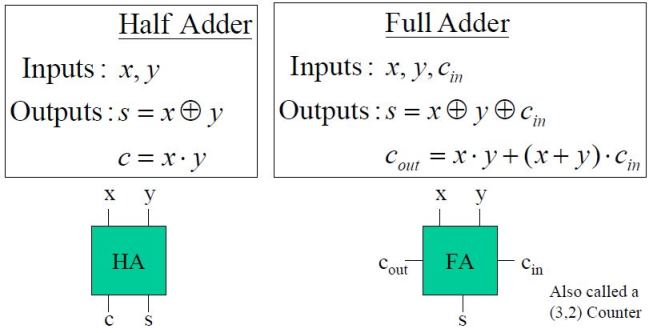
\includegraphics[width=0.7\linewidth]{img/img2/1}
\end{center}

$a_i$ and $b_i$ are two incoming operands, $s_i$ is the output sum bit,
$c_i$ and $c_{i+1}$ are input and output carry bits.
Boolean equations describing full adder are:

\begin{eqnarray*}
s_i=a_i \oplus b_i \oplus c_i\\
c_{i+1}=a_i \cdot b_i+a_i \cdot  c_i+b_i \cdot c_i\\
\end{eqnarray*}

In terms of performance two time delay can be employed:
$t_s$ is the delay between input and $s_i$, $t_c$ between input and carry out.
Usually $t_s > t_c$ since the critical path is most of the time along carry
propagation and so it is improved. With $t_{FA}$ we indicate the general delay
of full adder (therefore assuming $t_c \approx t_s$).

%%%%%%%%%%%%%%%%%%%%%%%%%%%%%%%%%%%%%%%%%%%%%%%%%%%%%%%%%%%%%%%%%%%%%%%%%%%%%%%%
%%%%%%%%%%%%%%%%%%%%%%%%%%%%%%%%%%%%%%%%%%%%%%%%%%%%%%%%%%%%%%%%%%%%%%%%%%%%%%%%
%%%%%%%%%%%%%%%%%%%%%%%%%%%%%%%%%%%%%%%%%%%%%%%%%%%%%%%%%%%%%%%%%%%%%%%%%%%%%%%%

\section{Ripple carry adder}
\begin{center}
  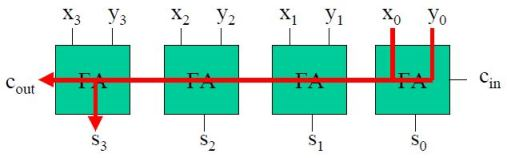
\includegraphics[width=0.7\linewidth]{img/img2/2}
\end{center}

Looking at this implementation complexity is linear with the number of bits,
critical path is the one along carry out propagation. Assuming $t_s>t_c$ c.p.is
the one along all carry out and going out from the last FA through its sum, so:

$$t_{cp}=(n-1)t_c+t_s$$

This architecture is modular and very simple, however its behavior in term of
performance is not very nice since delay is proportional to the number of bit.
A faster adder using this architecture cannot be build up.

%%%%%%%%%%%%%%%%%%%%%%%%%%%%%%%%%%%%%%%%%%%%%%%%%%%%%%%%%%%%%%%%%%%%%%%%%%%%%%%%
%%%%%%%%%%%%%%%%%%%%%%%%%%%%%%%%%%%%%%%%%%%%%%%%%%%%%%%%%%%%%%%%%%%%%%%%%%%%%%%%
%%%%%%%%%%%%%%%%%%%%%%%%%%%%%%%%%%%%%%%%%%%%%%%%%%%%%%%%%%%%%%%%%%%%%%%%%%%%%%%%

\subsection{Bit serial}

\begin{center}
  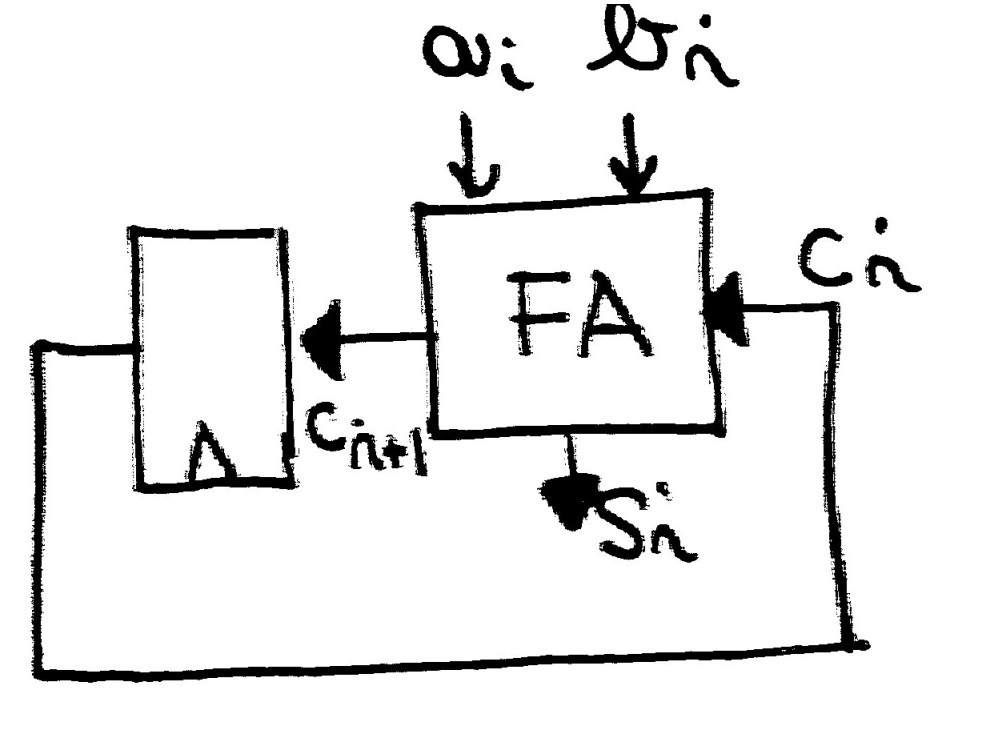
\includegraphics[width=0.5\linewidth]{img/img2/3}
\end{center}

It is the folded version of ripple carry adder (which is a parallel 
implementation). This is a nice example of decomposition: these last two 
implementations have different performance but the same ideal one. In the first
architecture in a single clock cycle the information propagates n FA, while in
the second n clock cycles are involved, meaning that parallel and serial have 
the same ideal throughput which is $\frac{1}{nt_{FA}}$.
Ideally performances are the same since we are neglecting delay along
interconnects, delay introduced by registers and so on.

%%%%%%%%%%%%%%%%%%%%%%%%%%%%%%%%%%%%%%%%%%%%%%%%%%%%%%%%%%%%%%%%%%%%%%%%%%%%%%%%
%%%%%%%%%%%%%%%%%%%%%%%%%%%%%%%%%%%%%%%%%%%%%%%%%%%%%%%%%%%%%%%%%%%%%%%%%%%%%%%%
%%%%%%%%%%%%%%%%%%%%%%%%%%%%%%%%%%%%%%%%%%%%%%%%%%%%%%%%%%%%%%%%%%%%%%%%%%%%%%%%

\subsection{Flag}
Often we also need to generate some flags.

\subparagraph{Zero}
Zero flag ($z$) is asserted when every sum bits are equal to zero, so:
$$z=\overline{s_0+s_1+...+s_{n-1}} $$

\subparagraph{Overflow}

An overflow condition occurs when:
\begin{itemize}
  \item $a_{n-1}=b_{n-1}=0 \qquad s_{n-1}=1 $ (operands expressed in CA2 are
    positive and the result is negative).
  \item $a_{n-1}=b_{n-1}=1 \qquad s_{n-1}=0$ (operands are negative and the
    result is positive).
\end{itemize}

In both cases we can identify the overflow condition by:
$$over=c_n  \oplus c_{n-1} $$
i.e. xor between carry in and carry out of full adder in most significant
position.

To justify this expression we notice that:
\begin{itemize}
  \item
    \subitem If $a_{n-1}=b_{n-1}$ then $s_{n-1}=c_{n-1}$.
    \subitem If $a_{n-1}=b_{n-1}=0$ then $c_n=0$.
  If overflow=1 then $s_{n-1}=1$ and $c_{n-1}=1$ therefore $c_n \oplus c_{n-1}=1$.

  \item
    \subitem If $a_{n-1}=b_{n-1}=1$ then $c_n=1$.
  If overflow=1 then $s_{n-1}=0$ and $c_{n-1}=0$ therefore $c_n \oplus c_{n-1}=1$.

\end{itemize}

\subparagraph{Sign bit}
Sign bit is computed as:

$$s=s_{n-1} \oplus over $$
meaning that if no overflow occurs sign bit equal to MSB bit, otherwise MSB has
to be complement since the result is wrong. Even in case of overflow we are able
to generate the correct sign bit.

%%%%%%%%%%%%%%%%%%%%%%%%%%%%%%%%%%%%%%%%%%%%%%%%%%%%%%%%%%%%%%%%%%%%%%%%%%%%%%%%
%%%%%%%%%%%%%%%%%%%%%%%%%%%%%%%%%%%%%%%%%%%%%%%%%%%%%%%%%%%%%%%%%%%%%%%%%%%%%%%%
%%%%%%%%%%%%%%%%%%%%%%%%%%%%%%%%%%%%%%%%%%%%%%%%%%%%%%%%%%%%%%%%%%%%%%%%%%%%%%%%

\subsection{Carry generation}
Before looking at different architecture, we need to consider a different way
to generate carry out.

\begin{center}
  \begin{tabular}{|c|c|c|c|c|}
    \hline
     $a_i$& $b_i$&    $c_i$&    $c_{i+1}$& Case\\
     \hline
      0&    0&    0&    0&    g\\
      0&    1&    0&    0&    a\\
      1&    0&    0&    0&    b\\
      1&    1&    0&    1&    e\\
      0&    0&    1&    0&    h\\
      0&    1&    1&    1&    c\\
      1&    0&    1&    1&    d\\
      1&    1&    1&    1&    f\\
    \hline
  \end{tabular}
\end{center}

Meaning that:

\begin{itemize}
  \item  In cases $a,b,c,d$ (i.e. $a_i$ different from $b_i$) then
    $c_{i+1}= c_i$, so we are in \textbf{propagate condition},
    carry out has not to be computed.
  $$p_i=a_i \oplus b_i$$

  \item In cases $e,f$ carry out is asserted independently from carry in,
    there is no propagation but $c_{i+1}$ is set to one by the output sum bit
    of the adder, so it is a \textbf{generate condition}. This implies that
    if $a_i=b_i=1$ then $c_{i+1}=1$ and so:
  $$g_i=a_i \cdot b_i$$

  \item In cases $g, h$ output carry is always zero independently from the 
    carry in, this is called \textbf{kill condition}. When $a_i=b_i=0$ 
    then $c_{i+1}=0$ and so:
  $$k_i=\overline{a_i+b_i}$$

\end{itemize}

Using $p_i, g_i, k_i$ it is possible to compute carry out bit.

%%%%%%%%%%%%%%%%%%%%%%%%%%%%%%%%%%%%%%%%%%%%%%%%%%%%%%%%%%%%%%%%%%%%%%%%%%%%%%%%
%%%%%%%%%%%%%%%%%%%%%%%%%%%%%%%%%%%%%%%%%%%%%%%%%%%%%%%%%%%%%%%%%%%%%%%%%%%%%%%%
%%%%%%%%%%%%%%%%%%%%%%%%%%%%%%%%%%%%%%%%%%%%%%%%%%%%%%%%%%%%%%%%%%%%%%%%%%%%%%%%

\section{Carry skip adder (CSKA)}

\begin{center}
  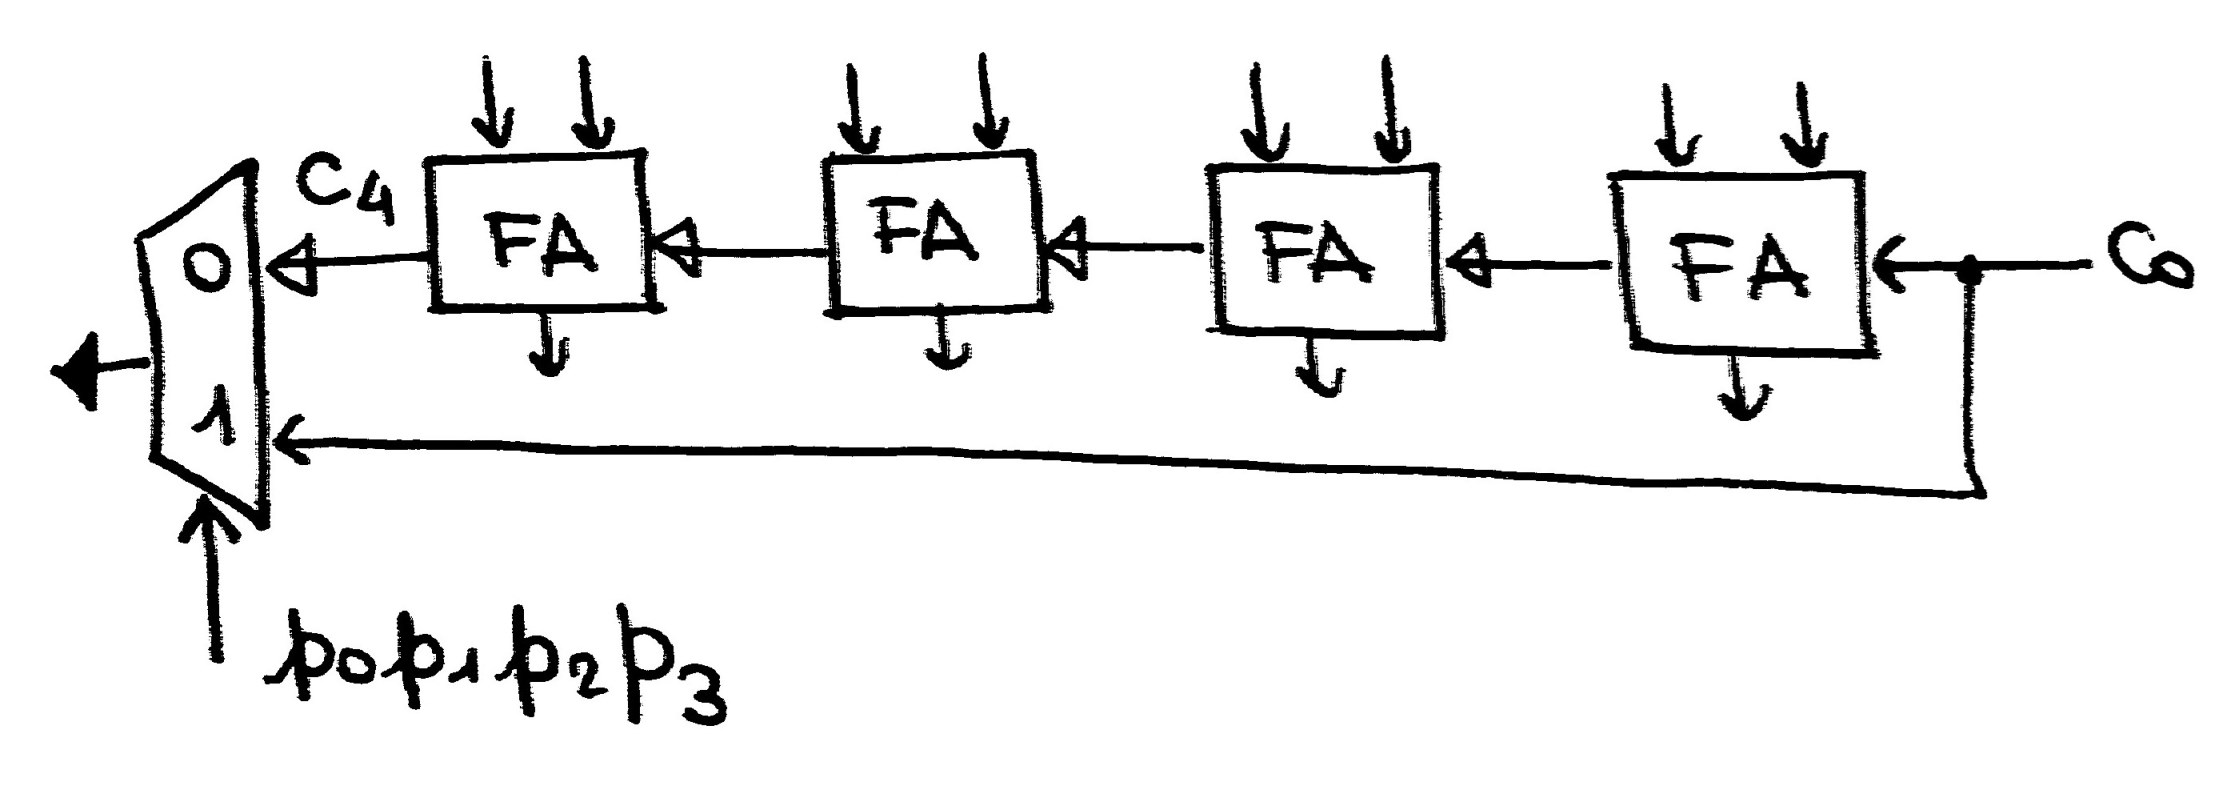
\includegraphics[width=0.7\linewidth]{img/img2/4}
\end{center}


Starting from RCA let's imagine to allocate also some additional gates to
calculate propagate bits for each stages. If $p_0=1$ it means that $c_1$
is equal to $c_0$, then if $p_1=1$ also $c_2$ will be equal to $c_1$;
therefore if all $p_i$ are equal to one the carry in propagates from input to
output. This is actually a particular case but it corresponds also to the worst
one for delay, in fact the situation for which the overall propagation of the
carries takes place corresponds to critical path and is therefore very
important.\\ Summarizing if $p_0\cdot p_1 \cdot p_2 \cdot p_3=1$ we can
anticipate the carry, otherwise it has to be computed. In any case, also
if $p_0=0$ it means that in stage 0 there will be a generate or a kill, so in
both cases the critical path has been reduced since it does not start from
$c_0$ but from $b_0$ or $a_0$. CSKA is faster only if we have the overall
propagation, otherwise the delay is a little bit greater due to multiplexer.

By applying this idea to a buffer adder:
\begin{center}
  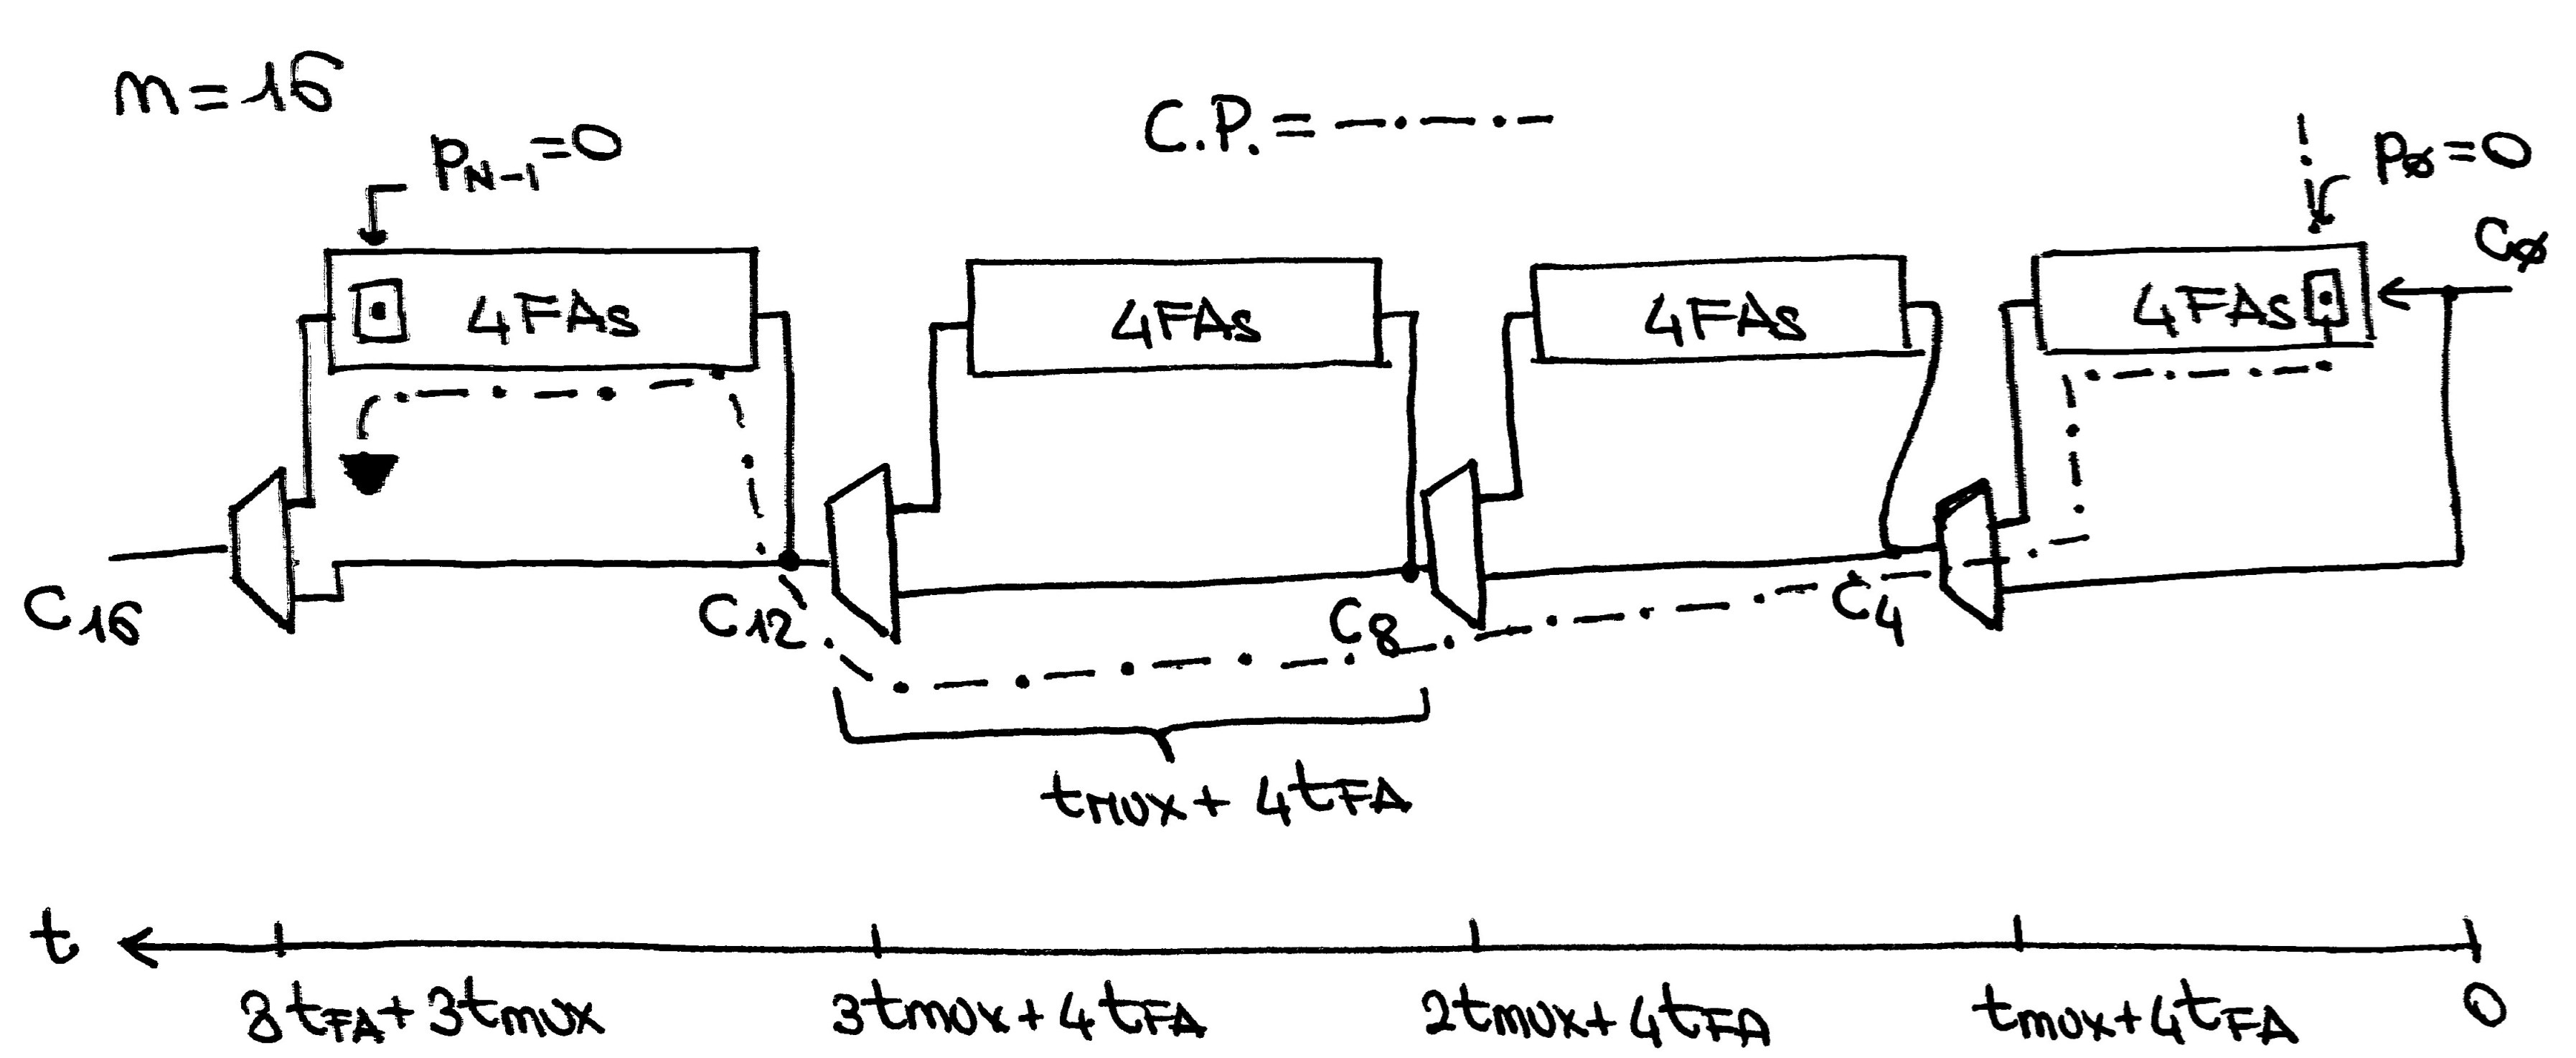
\includegraphics[width=0.8\linewidth]{img/img2/5}
\end{center}

The \textbf{Critical path} is the one with $p_0$ and $p_{n-1} = 0$. In other 
words in the case when all blocks except the first and last are in the progate 
condition.
In this condition all the RCA blocks in propagate condition have to wait for the
carry in comeing from the previous block, hence adding the $t_{mux}$ delay.
In case of not propagate condition the delay will be $t_{mux}$ anyway since the
RCA works in parallel with the one of the last block. \textit{The carry of the 
block is dependent on the pervious one only in case of propagation} (this is why
it can work in parallel).

Critical path is the one for which $p_0=0, p_1=p_2=p_3=1$ since any other
combination of $p_i$ leads to a shortest delay. Across the second block instead
the worst case is when all $p_i =1$, same thing occurs for block 3 and so on.
Regarding the last block if all $p_i=1$ then we will skip these adders and just
take the multiplexer delay, but if $p_{n-1}=0$ our carry will propagate up to
the last FA and then stop here so we have to pass through all FA of last adder.

At the MSB global delay is $t_d=8t_{FA}+3t_{mux}$.

In general for a $n$ bits adders, made up of $b$ blocks with $k$ bits each
(so $n=k \cdot b$), global delay can be expressed as:
$$t= (b-1)t_{mux} + 2 *k* t_{FA}= (b-1)t_{mux} + 2 \cdot \frac{n}{b} \cdot t_{FA}$$

Critical path goes through first and last blocks while in intermediate blocks
carry is always propagated (in this way we don't break the propagation from
input to output and don't consider a shortest critical path).\\
Taking the derivative of final expression and by setting it equal to zero,
the optimal number of blocks is the one for which:

$$b_{opt}=\sqrt{\frac{2nt_{fa}}{t_{mux}}}$$

Corresponding to optimal delay:

$$t_{min}=\sqrt{2nt_{TA}t_{mux}}-t_{mux}+2nt_{FA} \sqrt{\frac{t_{mux}}{2nt_{fa}}}$$

By the way $b_{opt}$ must be an integer number.

Delay is proportional to $\sqrt{n}$ so the behavior is not linear like RCA and
growing speed is much slower than previous architecture.\\

Some additional improvements to CSKA can be performed by assuming to have
defined an optimal number for $b$. Minimizing $k$ is useful to reduce the
second delay contribution while reducing $b$ we can reduce the first term;
but unfortunately we cannot modify independently $k$ and $b$ because they are
related. If we image that every block may have a different number of FA we are
introducing a freedom degree. The idea is that internal blocks are bigger than
starting and lasting one, so we can reduce $k_0t_{FA}$ and since the internal
$k_j$ are bigger there will be less blocks leading to a smaller delay
associated to multiplexers.
\begin{center}
  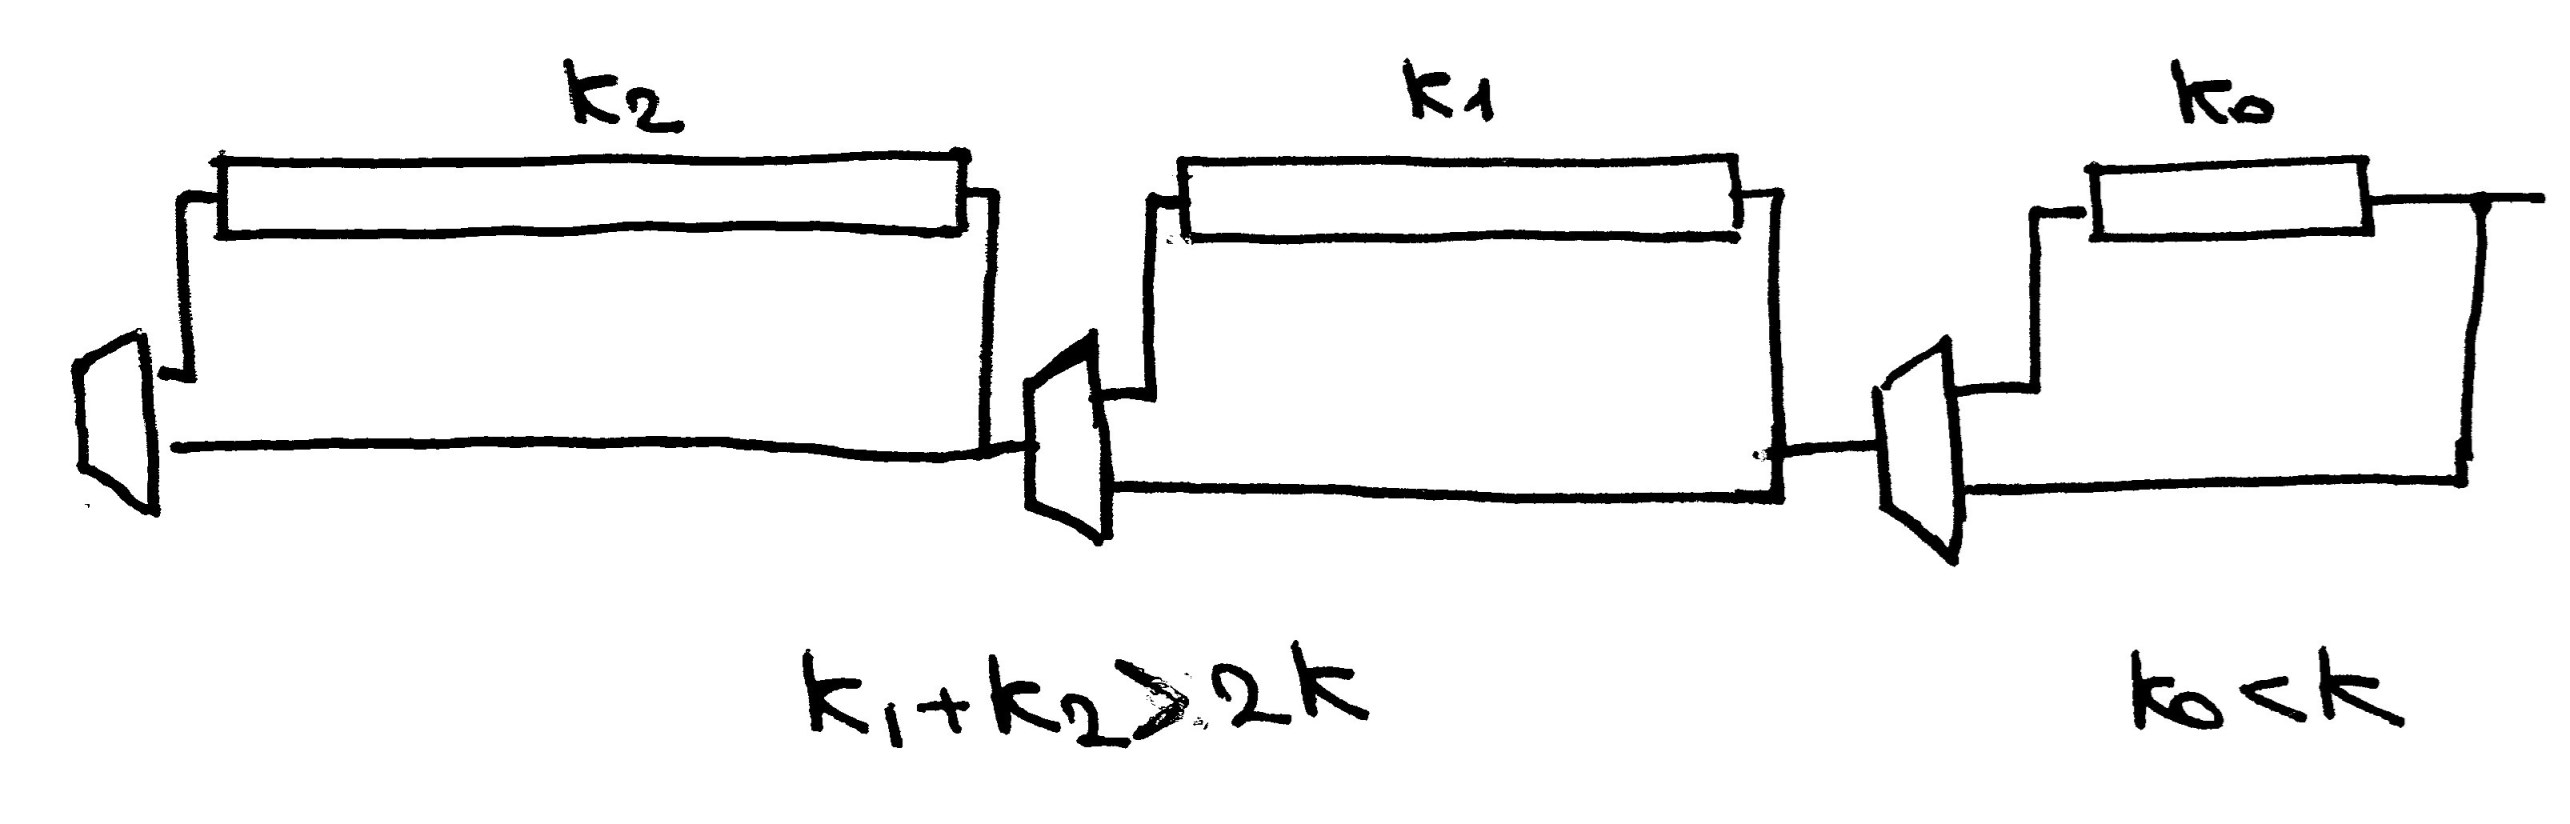
\includegraphics[width=0.7\linewidth]{img/img2/6}
\end{center}


Delay is still proportional to $\sqrt{n}$ but the coefficient is smaller than
before, the idea of skipping blocks can be further exploited improving
coefficient but not the kind of function.

%%%%%%%%%%%%%%%%%%%%%%%%%%%%%%%%%%%%%%%%%%%%%%%%%%%%%%%%%%%%%%%%%%%%%%%%%%%%%%%%
%%%%%%%%%%%%%%%%%%%%%%%%%%%%%%%%%%%%%%%%%%%%%%%%%%%%%%%%%%%%%%%%%%%%%%%%%%%%%%%%
%%%%%%%%%%%%%%%%%%%%%%%%%%%%%%%%%%%%%%%%%%%%%%%%%%%%%%%%%%%%%%%%%%%%%%%%%%%%%%%%

 \section{Carry select adder (CSA)}
 In this architecture a brute force approach is employed since we try to stop
 the complete propagation of carry. Starting from a 4 bits RCA and by putting
 another 4 bits RCA for the second block, we must to wait the propagation of
 carry along the first RCA. Since we want to avoid it, for the second block we
 allocate two identical blocks, where for one of them we assume that $c_{in}=0$
 and for the other one that $c_{in}=1$, in this way there are 3 RCA working in
 parallel. The idea is to allocate additional adders to compute all possible
 cases and then choose the correct one.

\begin{center}
  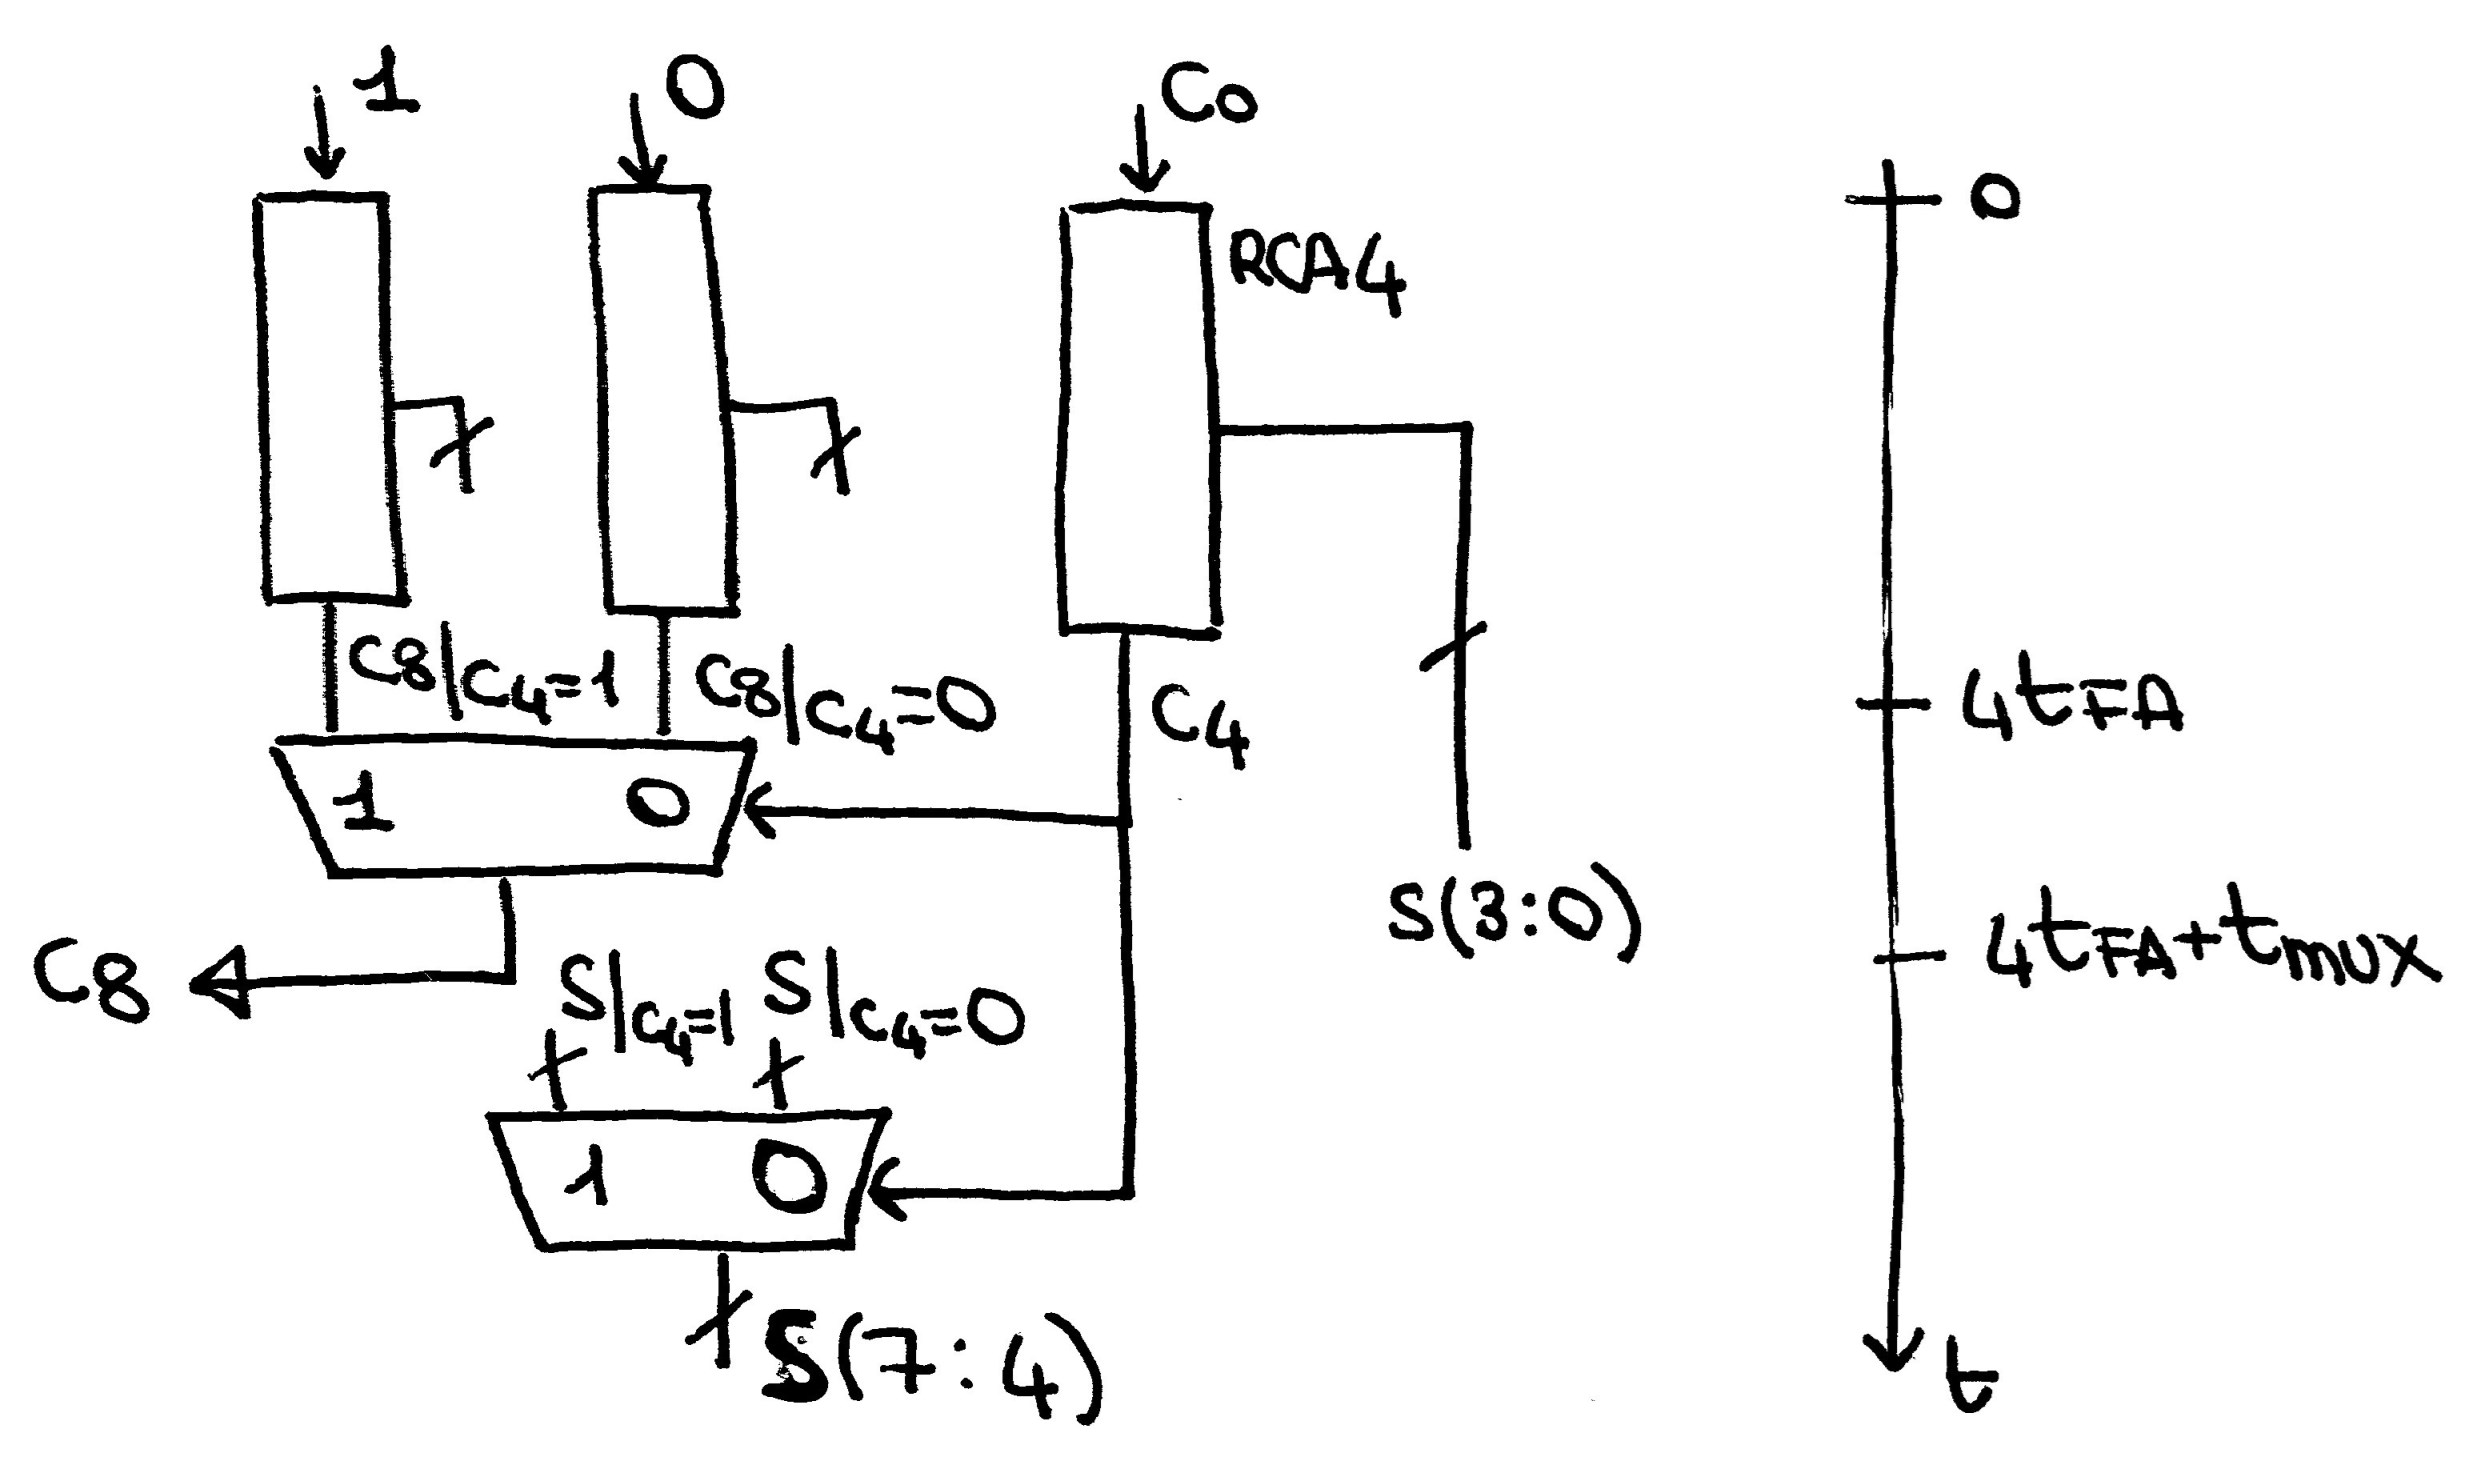
\includegraphics[width=0.7\linewidth]{img/img2/7}
\end{center}


 Two different architectures can implement this idea in a real full adder.

%%%%%%%%%%%%%%%%%%%%%%%%%%%%%%%%%%%%%%%%%%%%%%%%%%%%%%%%%%%%%%%%%%%%%%%%%%%%%%%%
%%%%%%%%%%%%%%%%%%%%%%%%%%%%%%%%%%%%%%%%%%%%%%%%%%%%%%%%%%%%%%%%%%%%%%%%%%%%%%%%
%%%%%%%%%%%%%%%%%%%%%%%%%%%%%%%%%%%%%%%%%%%%%%%%%%%%%%%%%%%%%%%%%%%%%%%%%%%%%%%%

\subsection{Linear approach}

Assuming n=16, k=4 bits/blocks

\begin{center}
  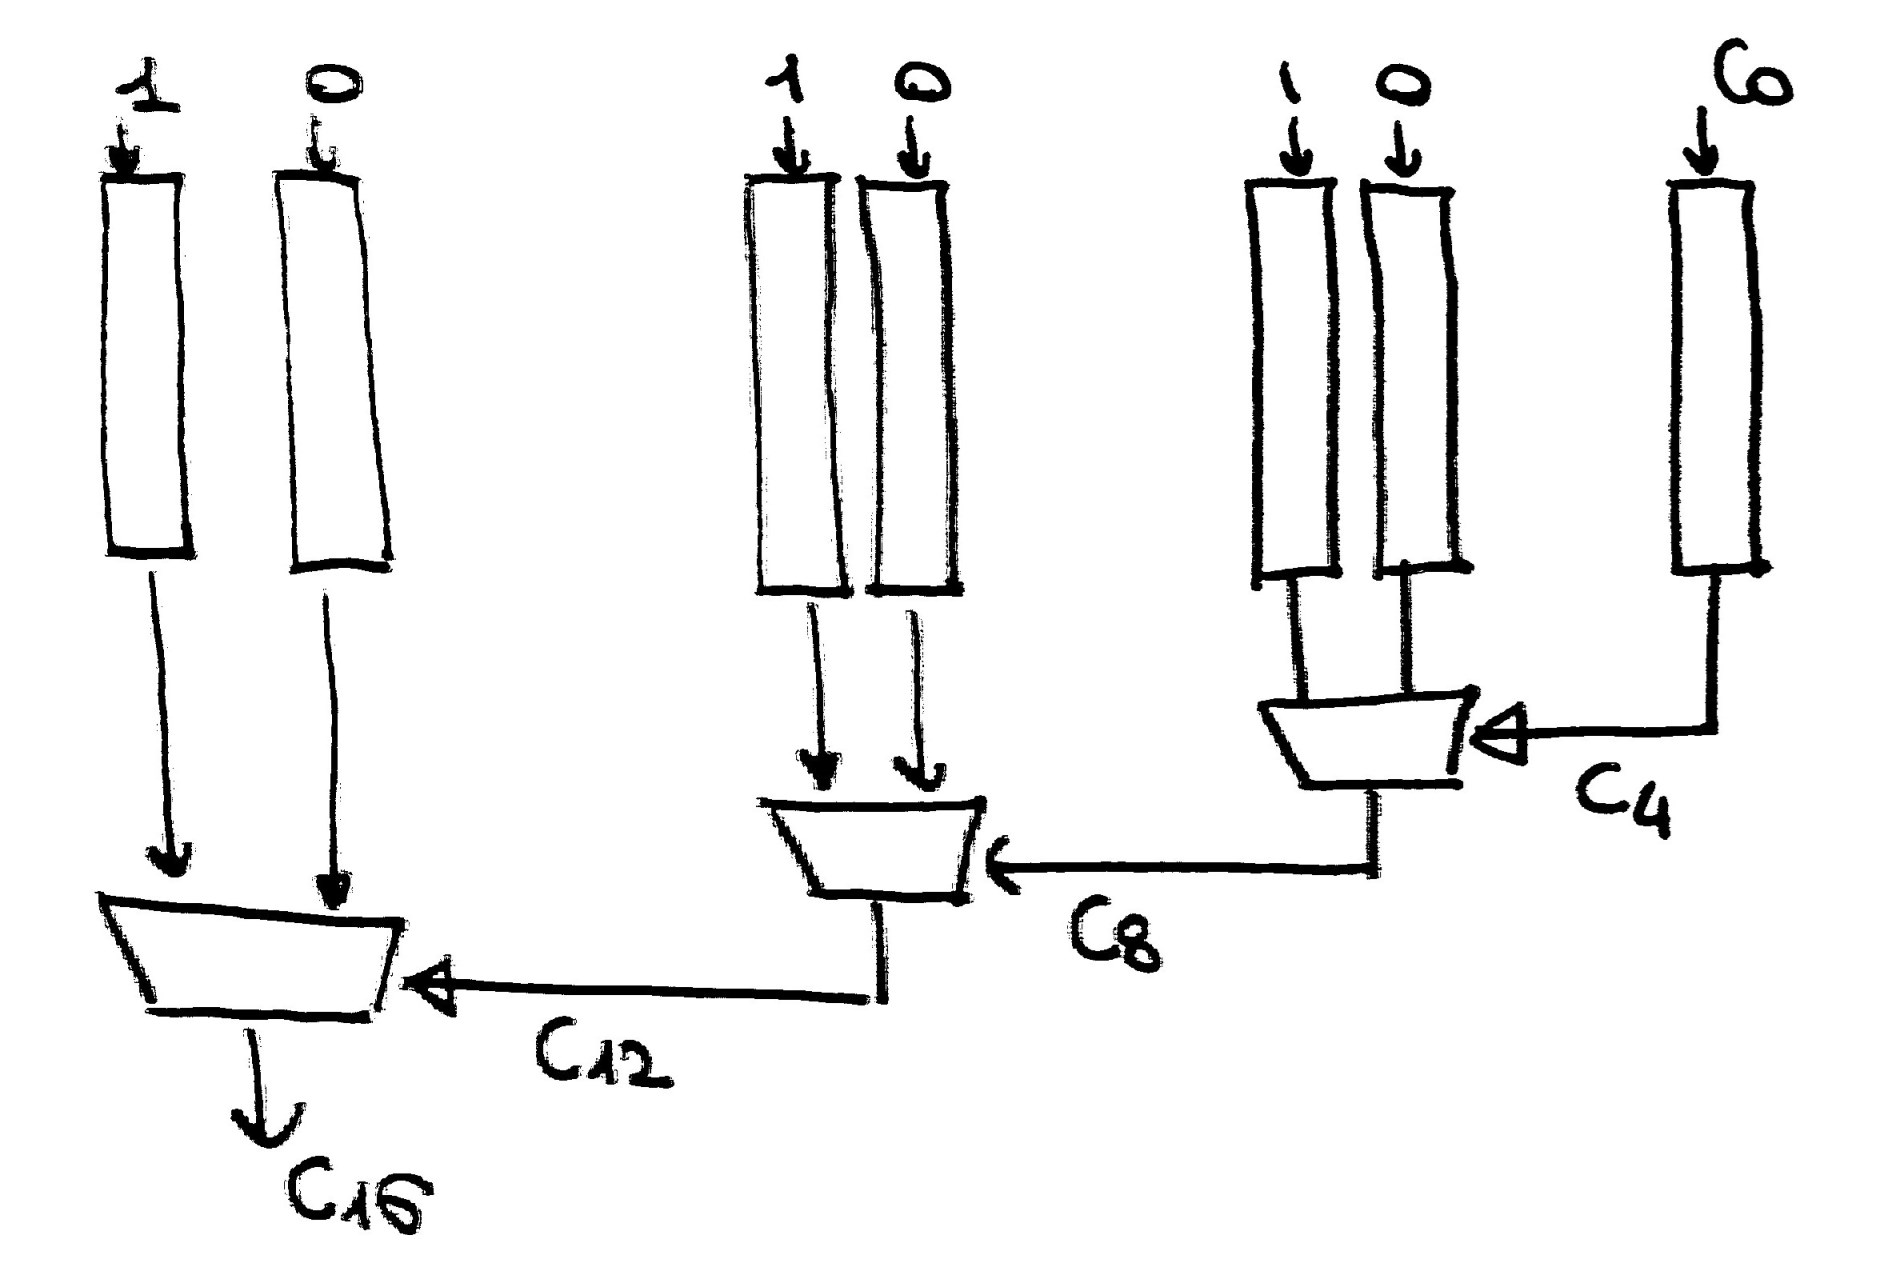
\includegraphics[width=0.7\linewidth]{img/img2/8}
\end{center}

 We allocate two RCA-4 bit for each block/stage acting in parallel. This is a
 linear approach since the delay increases linearly with the number of
 multiplexer. With $n=16$ the global delay is $t_d=4t_{fa}+3t_{mux}$. For a
 generic $n$ bits adder made up of $b$ blocks with $k$ bits/blocks, the total
 delay is:

 $$t=kt_{fa}+(b-1)t_{mux}$$

Since $b=n/k$ we can derive wrt $k$ to find the optimal solution:

$$t=kt_{fa}+(\frac{n}{k}-1)t_{mux}$$

By fixing $n$ and optimizing with respect to $k$:

$$ \frac{\partial t}{\partial k} = 0 \longrightarrow  t_{fa}-
\frac{n}{k^2} t_{mux}=0 \longleftrightarrow k=\sqrt{\frac{nt_{mux}}{t_FA}} $$

By choosing the proper $k$ we can reach better performances of a CSKA with
double area, so design constraints are the key to choose the proper one.\\

In this architecture every block works in parallel and complete its task at
the same time of the other ones but then we have to wait for three multiplexer.
By choosing blocks with increasing number of FA, it is possible to mitigate the 
mux delay having more or less the same area (\textbf{Root CSA}). (Compensation 
consist in adding a FA more or less every two muxes).
In this way we obtain a smaller coefficient but the dependency
is always sub-linear.

%%%%%%%%%%%%%%%%%%%%%%%%%%%%%%%%%%%%%%%%%%%%%%%%%%%%%%%%%%%%%%%%%%%%%%%%%%%%%%%%
%%%%%%%%%%%%%%%%%%%%%%%%%%%%%%%%%%%%%%%%%%%%%%%%%%%%%%%%%%%%%%%%%%%%%%%%%%%%%%%%
%%%%%%%%%%%%%%%%%%%%%%%%%%%%%%%%%%%%%%%%%%%%%%%%%%%%%%%%%%%%%%%%%%%%%%%%%%%%%%%%

\subsection{Logarithmic approach}
To obtain a logarithmic law a binary tree organization is required. Assuming
that $N$ is equal to the adder parallelism, initially we divide N into two
equal parts $(0 \rightarrow \frac{N}{2}+1) (\frac{N}{2} \rightarrow N-1)$,
for the lowest part we allocate just one block while for the second we allocate
two equal blocks working in parallel. Then we proceed in the same way by
dividing one of this three block and reusing carry select approach, so for the
least significant block we apply exactly the same scheme (same topology, only
indexes change). Same thing occurs for most significant bits since we can split
into N/4 bits blocks. Carry out it's determine by $c_{\frac{3n}{4}}$ so we need
to allocate two multiplexers having same inputs but different selecting signal.

\begin{center}
  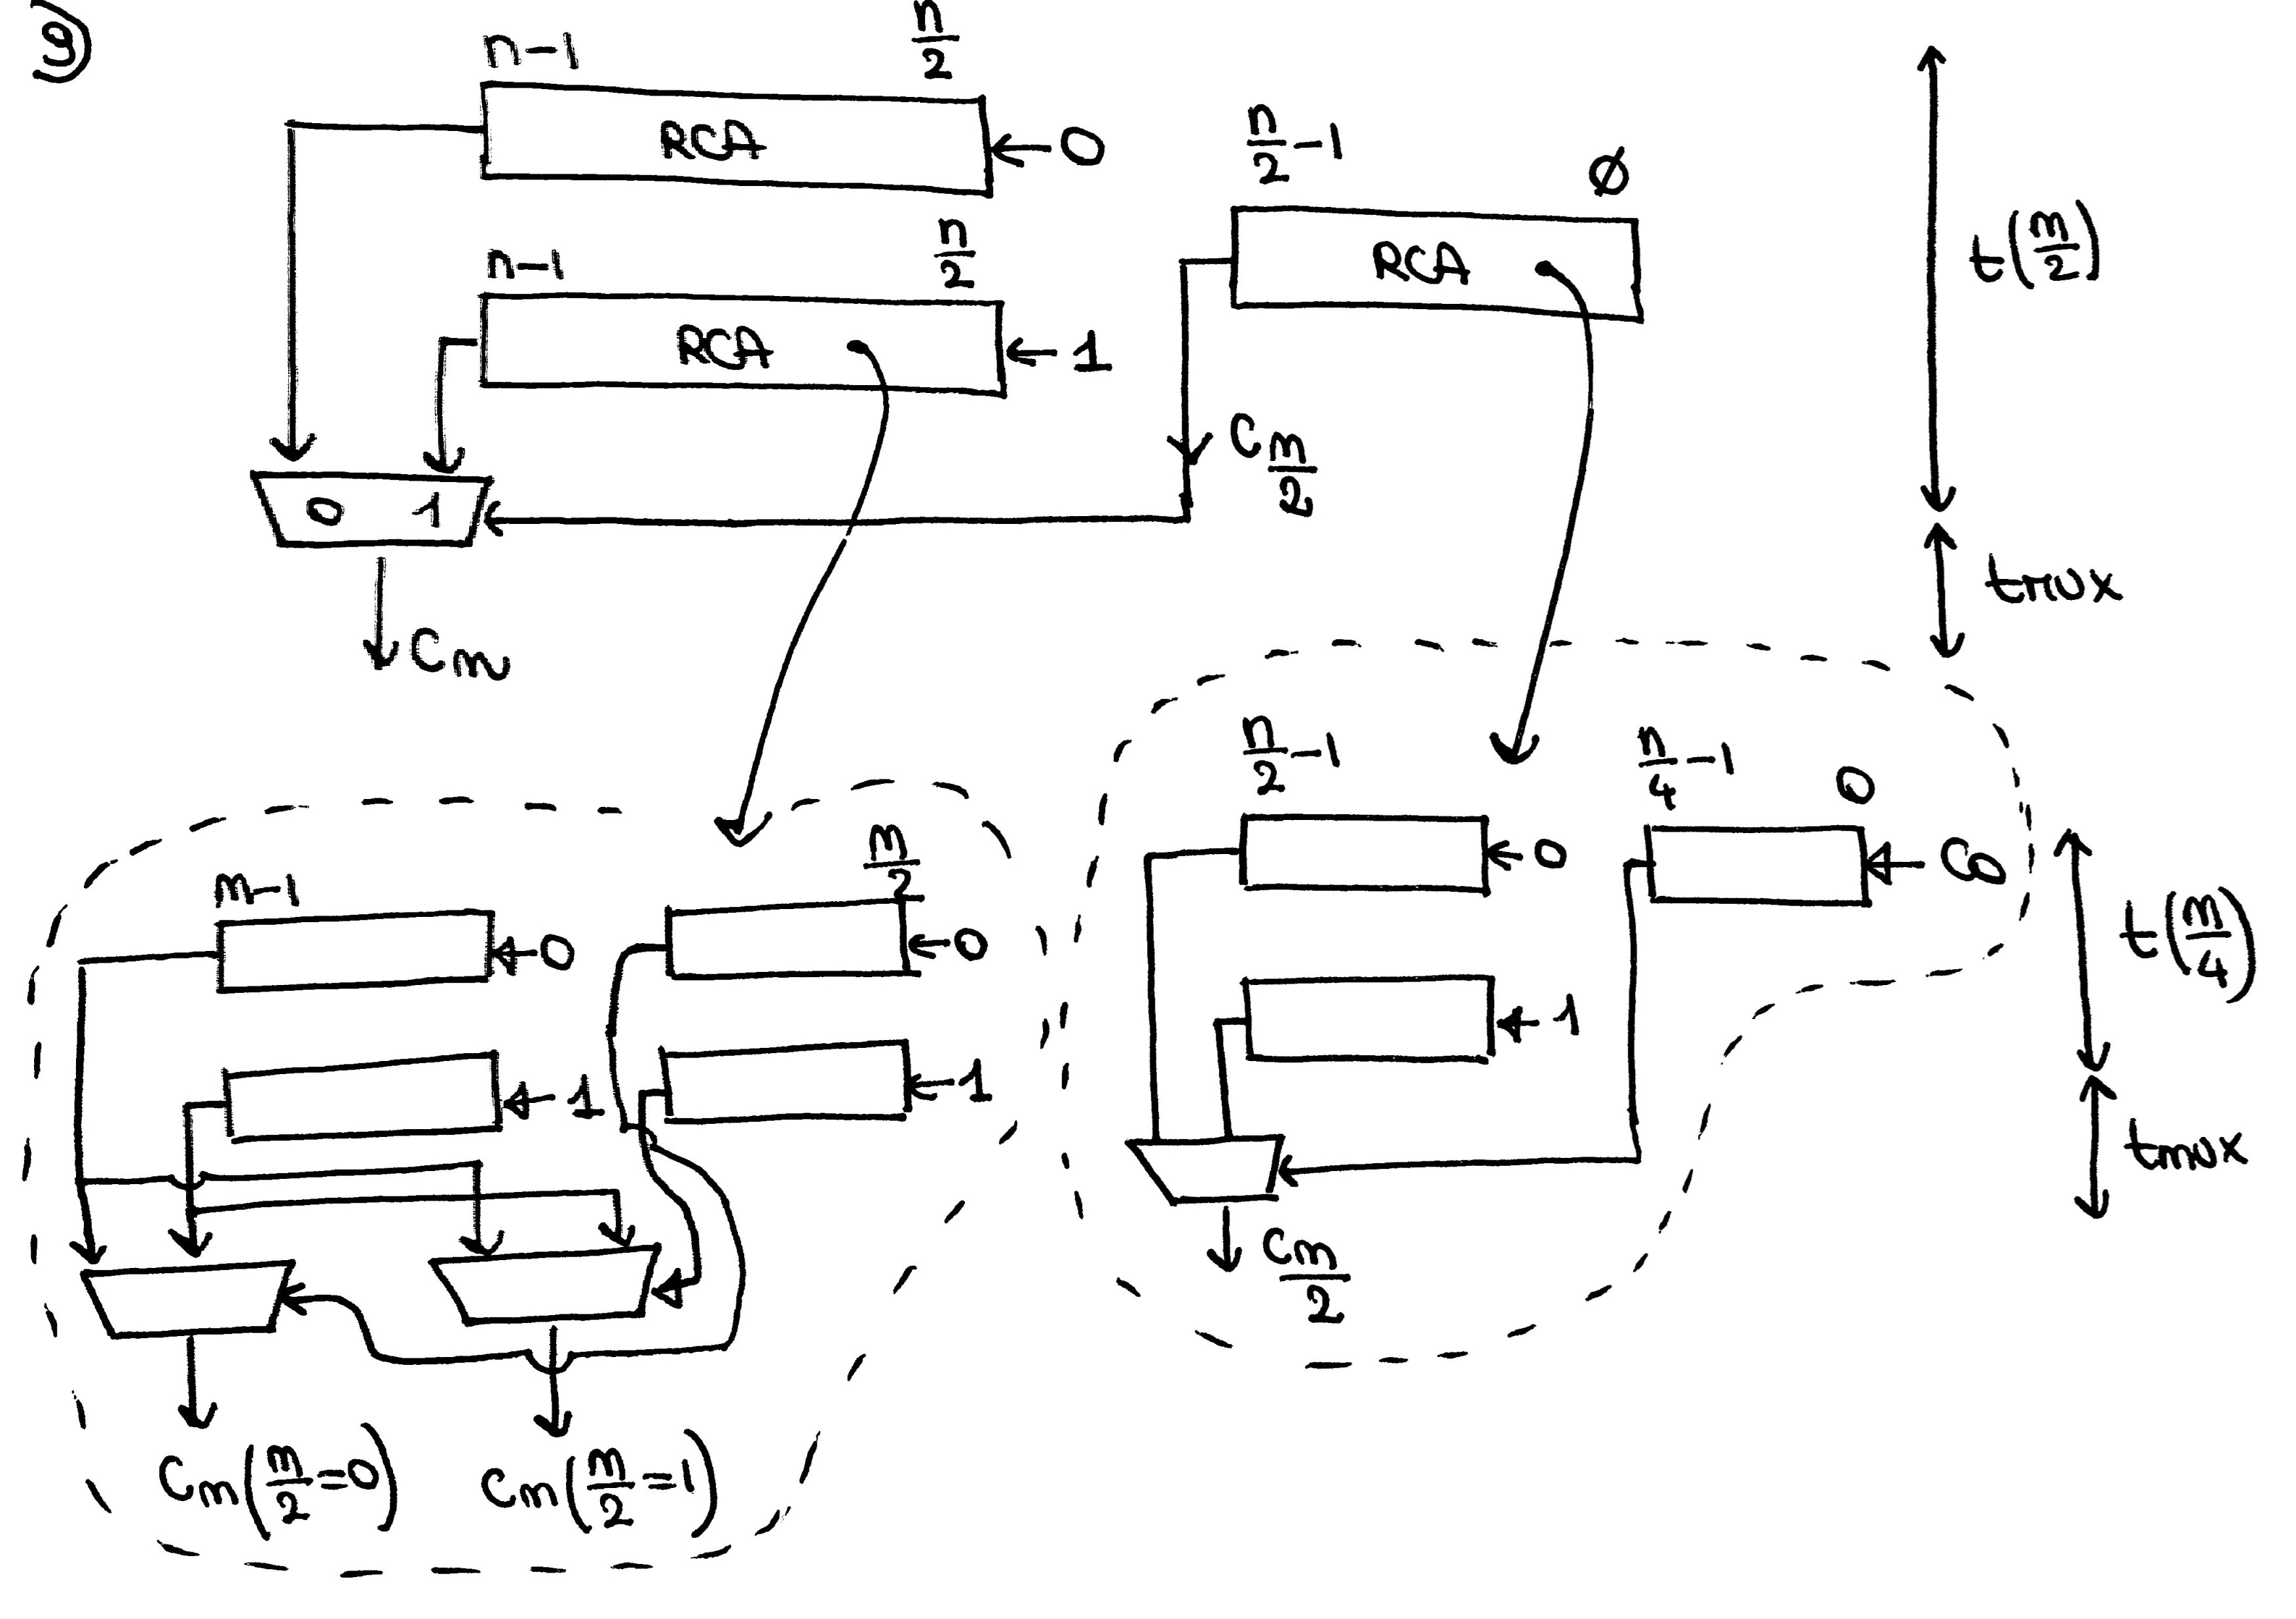
\includegraphics[width=0.7\linewidth]{img/img2/9}
\end{center}


Every time we perform this decomposition we add a new multiplexer layer.
Applying this approach more than one time:

\begin{center}
  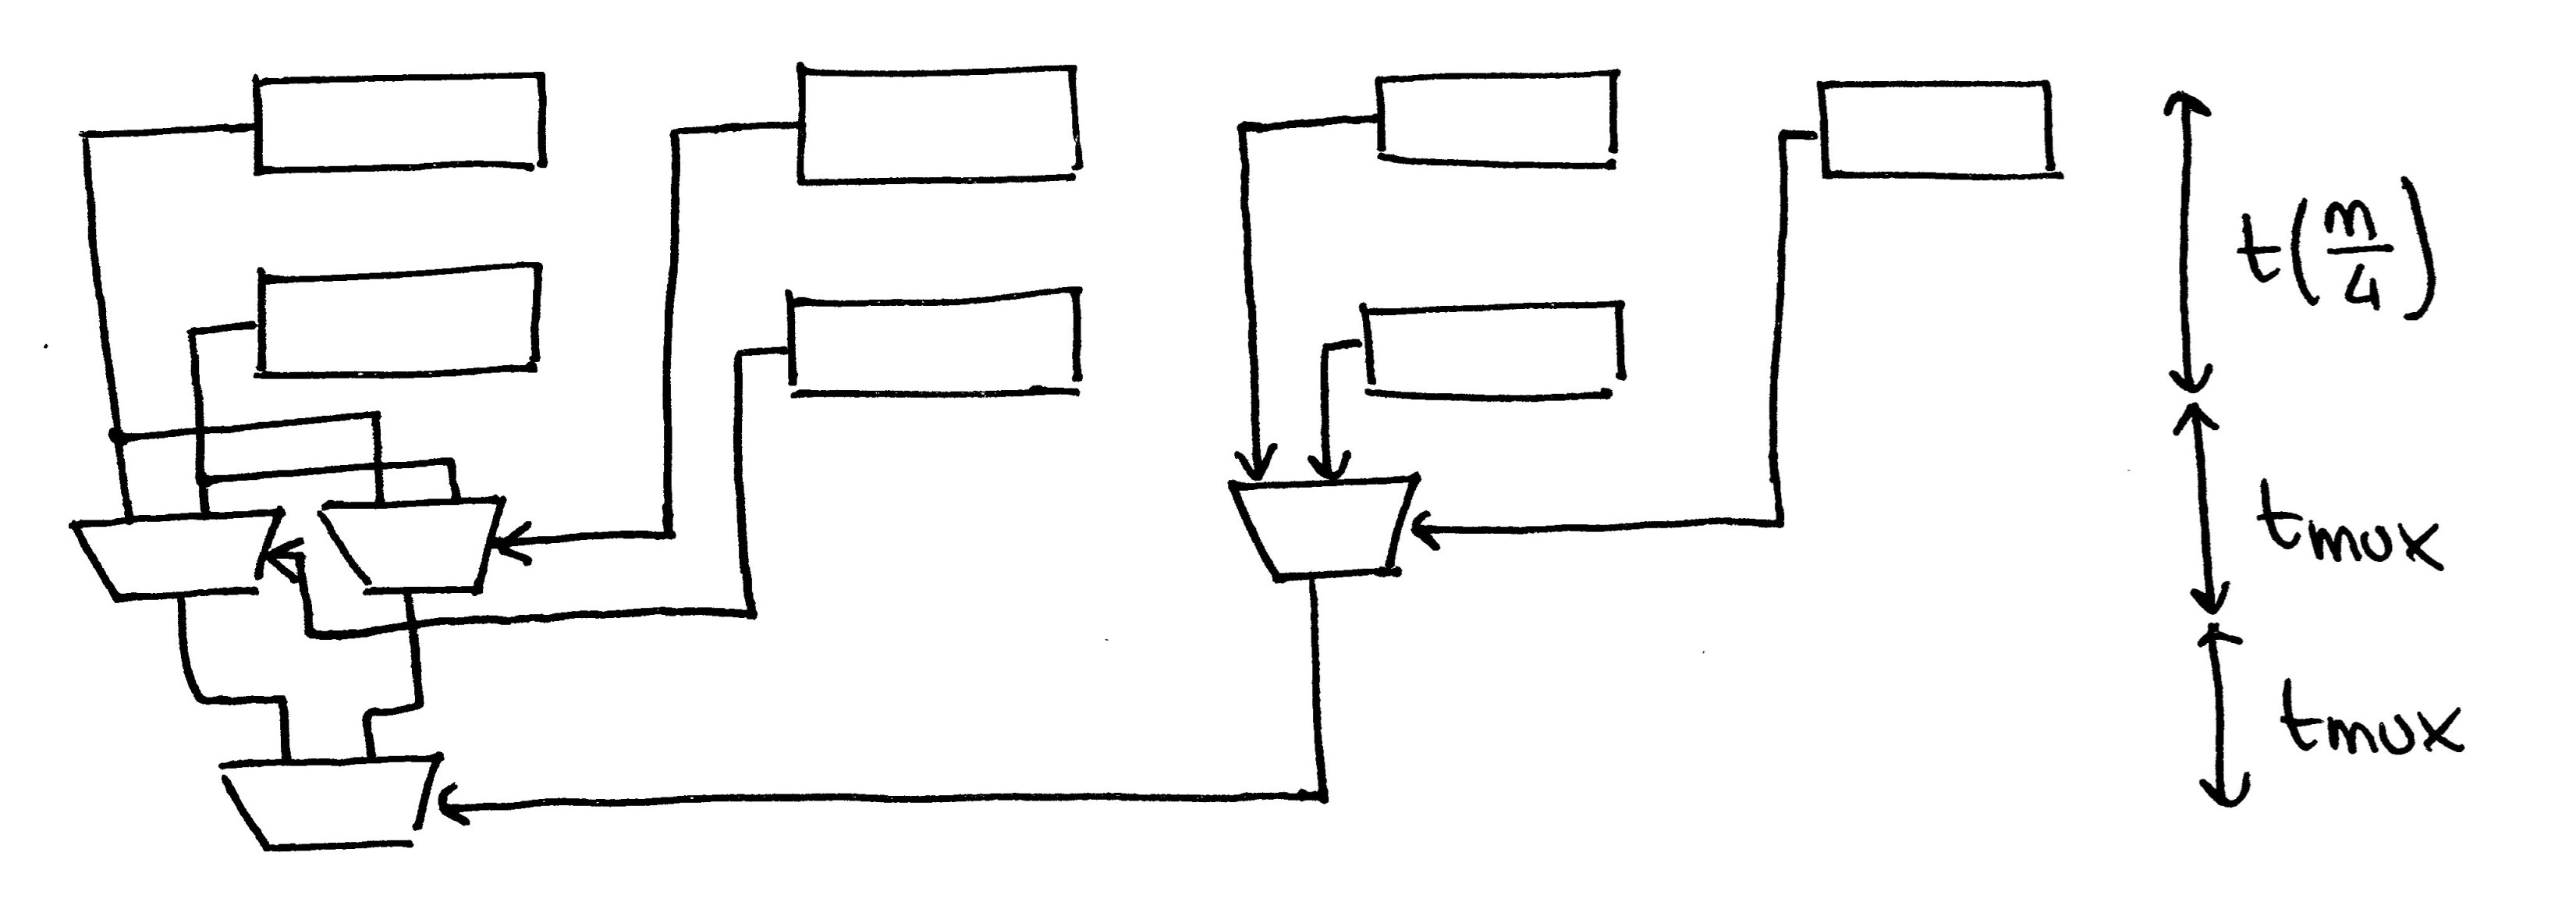
\includegraphics[width=0.7\linewidth]{img/img2/10}
\end{center}


By calling $k$ the amount of decomposition adopted, $k$ is also equal to
multiplexer levels, the delay of each level can be expressed as:

\begin{center}
\begin{tabular}{|c|c|}
  \hline
  $t(N/2)+t_{mux}$&     $1^{st}$ level\\
  $t(N/4)+2t_{mux}$&    $2^{nd}$ level\\
  $t(N/8)+3t_{mux}$&    $3^{rd}$ level\\
  $t(N/2^i)+it_{mux}$&  $i^{th}$ level\\
  \hline
\end{tabular}
\end{center}

Decomposition can be exploited up the point where each block is a single full
adder (working on just one bit), at this point $t_{FA}=t(1)=t(n/2^h)$
where $n=2^h \rightarrow h=log_2 n$
and so the total amount can be written as:

$$t(n)=t_{fa}+log_2(n) t_{mux}$$

\subparagraph{Example: 16-bit adder}

In this case first three blocks are working on two bit each. In terms of speed
it's very powerful but we need to allocate 2x full adders and multiplexer, so
we are looking for other solutions. One of the most popular is the
carry look-ahead adder.

%%%%%%%%%%%%%%%%%%%%%%%%%%%%%%%%%%%%%%%%%%%%%%%%%%%%%%%%%%%%%%%%%%%%%%%%%%%%%%%%
%%%%%%%%%%%%%%%%%%%%%%%%%%%%%%%%%%%%%%%%%%%%%%%%%%%%%%%%%%%%%%%%%%%%%%%%%%%%%%%%
%%%%%%%%%%%%%%%%%%%%%%%%%%%%%%%%%%%%%%%%%%%%%%%%%%%%%%%%%%%%%%%%%%%%%%%%%%%%%%%%

\section{Carry look-ahead adder}
 Recalling generate and propagate bit:

 \begin{eqnarray*}
 g_i=a_i \cdot b_i\\
 p_i=a_i \oplus b_i\\
 c_{i+1}=g_i+p_i \cdot c_i\\
 \end{eqnarray*}

Output carry is asserted either if the input carry is equal to one and we are
in propagate either if we are in generate (independently from input carry).
Since $p_i$ is now used only to calculate $c_{i=+1}$, the use of a XOR is
redundant, hence a OR is sufficient.As a consequence now $p_i$ does not
represent anymore a real propagate condition. Anyway $c_{i+1}=g_i+p_i \cdot c_i$
is still valid.\\
In principle every level of carry can be obtained by two-level logic:

\begin{center}
  \begin{tabular}{|c|c|l|}
    \hline
    Level& Carry out& Expression\\
    \hline
     0&   $c_0$&  \\
    1&    $c_1$& $g_0+p_0c_0$\\
    2&    $c_2$& $g_1+p_1c_1=g_1+p_1(g_0+p_0c_0)=g_1+p_1g_0+p_1p_0c_0$\\
    3&    $c_3$& $g_2+p_2g_1+p_2p_1g_0+p_2p_1p_0c_0$\\
    \hline
  \end{tabular}
\end{center}

Apparently at any level the delay is the one of two gates. However, in CMOS 
logic a 4-input OR is not so fast. Since at each further level there will be one
more input this implementation can be applied up to 4-5 level. Organizing a 
little bit better the computing of generate/propagate 
we can obtain some improvements.\\

Looking at $g_i$ it's a 1 bit signal which is asserted if we expect to have $c_{i+1}=1$ because it's generated by full adder in position $i$. Instead a working on a single bit we define a block generate signal which is high if the carry is generated inside that block. Formally we call:

\begin{itemize}
  \item \textbf{Block propagate}: the notation $P_{0,1}=p_0p_1$ corresponds to consider {0,1} as range, inside which there is a propagation from input of FA 0 to output of FA 1 if both full adders are in propagate condition.
  \item \textbf{Block generate}: the notation $G_{0,1}=g_1+g_0 \cdot p_1$ corresponds to the condition in which there is a generation in FA1 or generation in FA0 and propagation in FA1.
\end{itemize}

\begin{center}
  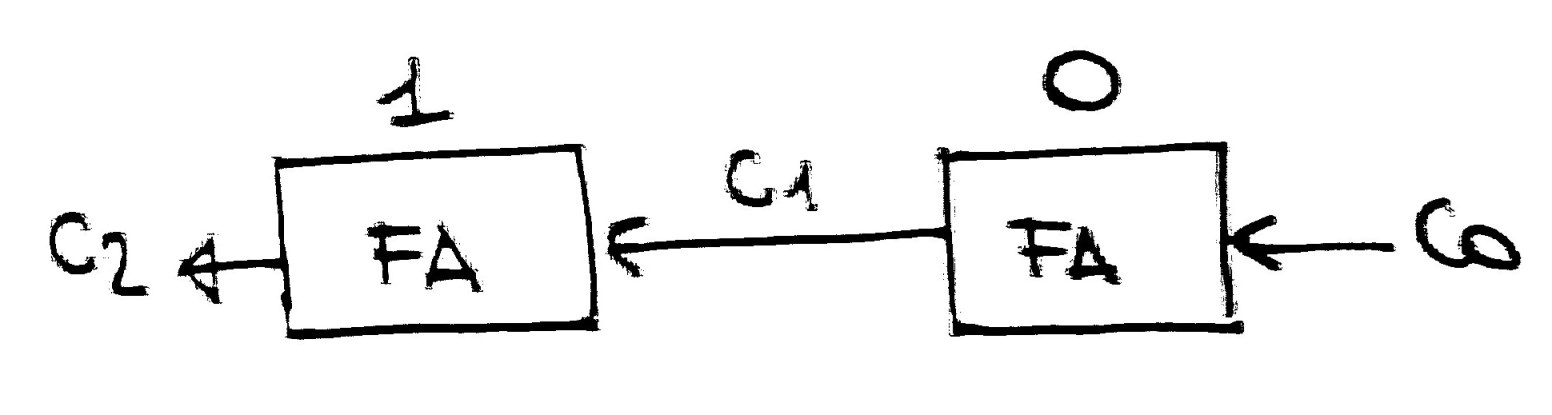
\includegraphics[width=0.6\linewidth]{img/img2/11}
\end{center}


These definitions can be applied to any level block where block size is arbitrary. In general it is possible to write:
$$P_{i,j}=p_ip_{i+1}p_{i+2}..p_{j}$$
$$G_{i,j}=g_j+g_{j-1}p_j+g_{j-2}p_{j-1}p_j$$

A very useful situation is when we have to compute carry out for a block which has been subdivided, meaning that starting from range (i, j) we split it into (i, k-1) and (k, j) (assuming j greater than i), in this case we can write:

$$P_{i,j}=P_{i, k-1} \cdot P_{k, j}$$
$$ G_{i, j}=G_{k, j}+G_{i, k-1}\cdot P_{k, j}$$

These new propagate/generate representations can be exploited to implement a tree-like topology capable of obtaining a logarithmic dependency of the delay in function of N.\\

Defining the following basic blocks:

\begin{center}
  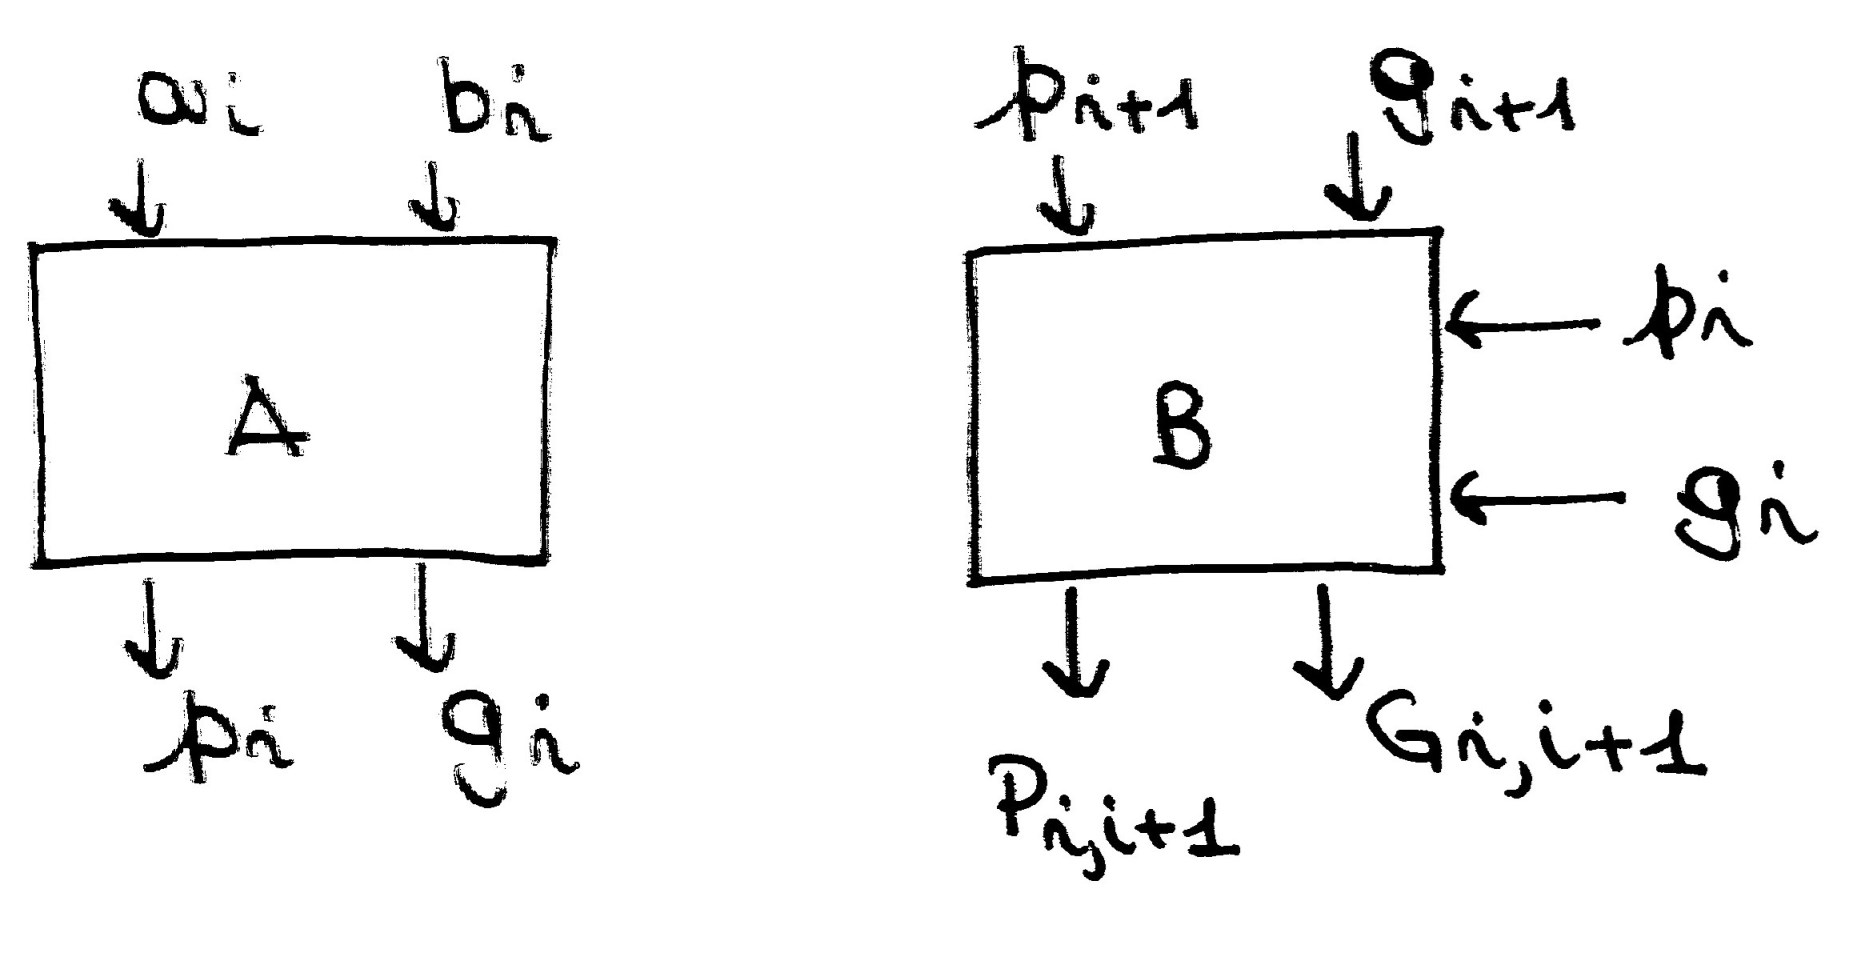
\includegraphics[width=0.6\linewidth]{img/img2/12}
\end{center}

By using them we can organized the addition in the following way:

 $\#$fig 13 (solo matita)

In first level propagate and generate are the classic bits, in second level using block B we are mixing two 2 propagate/generate and generating at the output 4 signal blocks.

We are building up a tree system where range length is doubled at each level. The key difference with respect to long boolean equations is in the use of block system, in this way we don't have to pass through a linear structure but through a logarithmic one. If we have to pass from 8 to 16 or 16 to 32 bit adders we just have to add one more level (no double of critical path). However we still have to compute $c_7$, to perform this the functionality of block A is extended so we suppose that starting from a $c_i$, it can also compute $s_i$. Moreover also B block must be slightly modified:
\begin{center}
  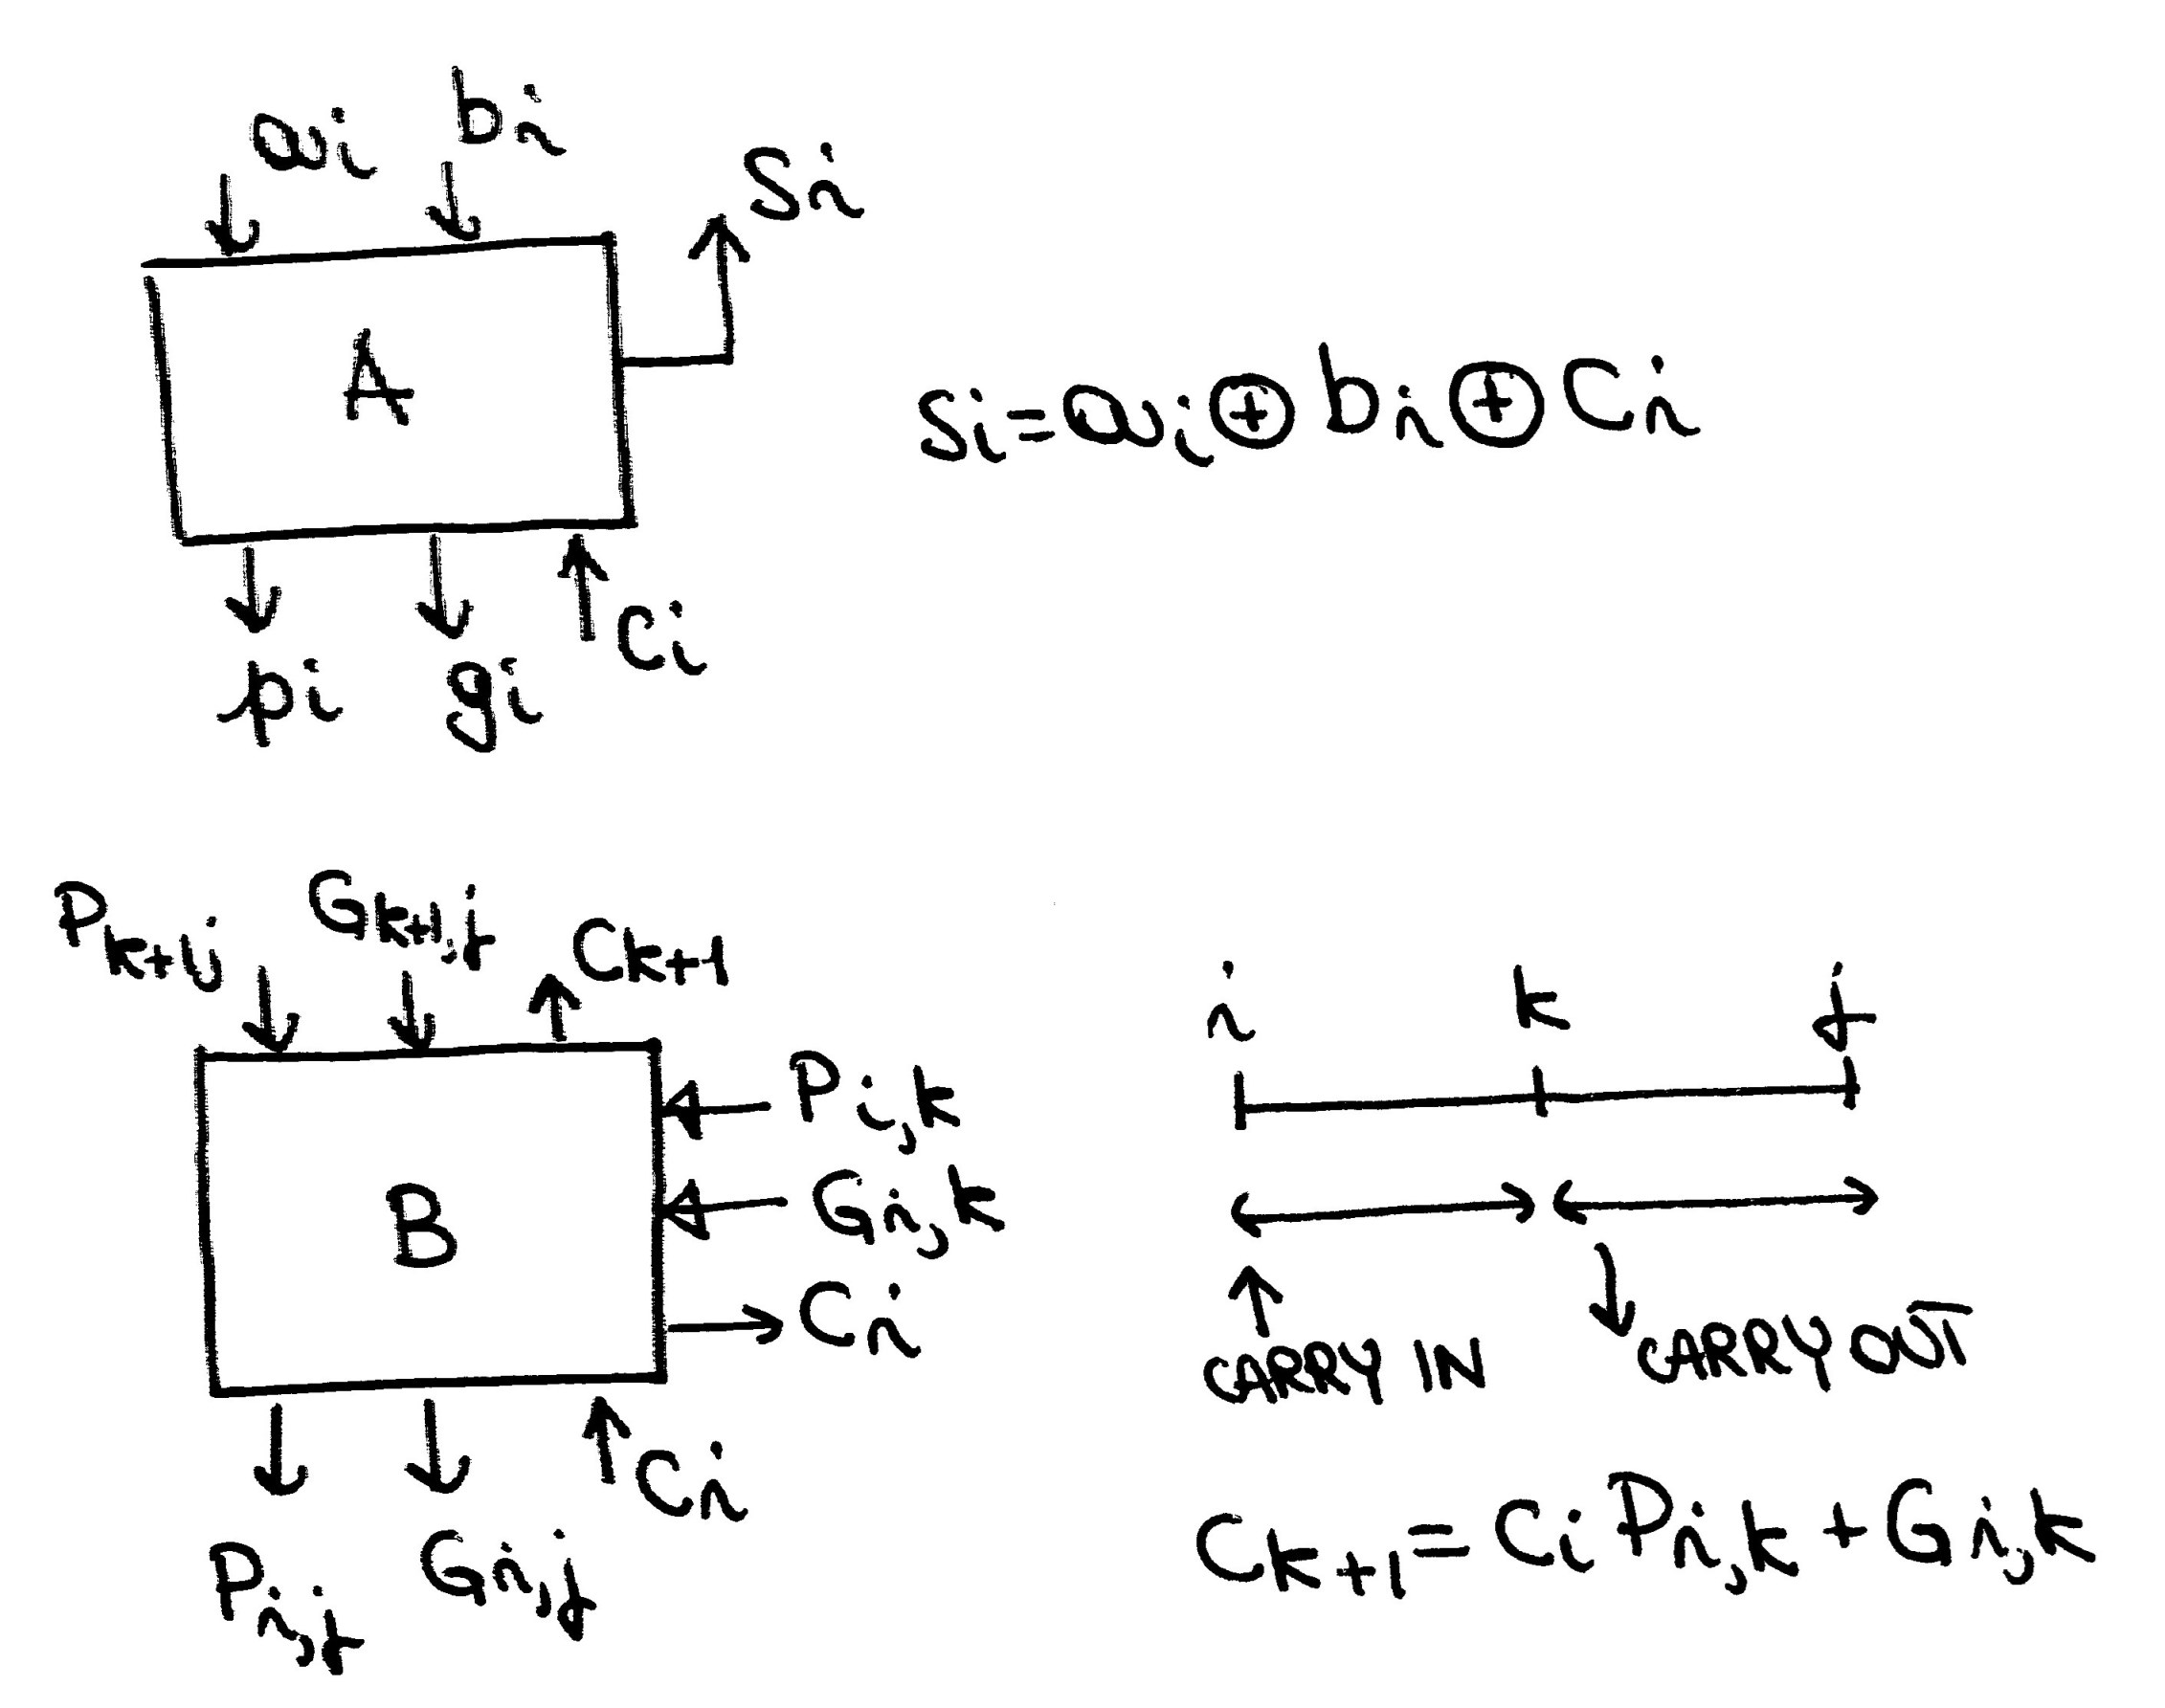
\includegraphics[width=0.6\linewidth]{img/img2/14}
\end{center}

B block is implementing two tasks: from top to bottom are the original equations, from bottom to top it generates the carry out in the least significant part.

If we modify the previous scheme using this extended blocks, we obtain:
\#fig 13 a colori

We have the possibility to generate all G, P by going from top to bottom in the tree, then coming back from bottom to top we are able to compute all $c_i$ and finally the sum bits. Since we have to go through this structure twice So we need to go through this structure twice, therefore the corresponding delay will be:

$$t=t_{A \downarrow} + ((log_2 n)-1) t_{B \downarrow} + (log_2n)t_{B \uparrow}+t_{A \uparrow}$$

where the last level has to be considered only in bottom-up direction.

What is important to notice is that delay increases with the logarithm of n and that we don't need to double full adders but just to add resources inside block A (their number is growing linearly with N) and inside block B (more difficult but growing logarithmic with N).

The overall architecture is tree-like but there is a double path (from top to bottom and then from bottom to top), so the coefficient of logarithm is quite large: parallel prefix adders try to improve this point.

\section{Parallel prefix adder (PPA)}

In general starting from $N$ numbers $x_0, x_1, ...,x_{N-1*}$ the point we are addressing is to find a network that can efficiently compute $x_0, x_0+x_1, x_0+x_1+x_2, ...$. We want to find all possibles sum from $i=0$ to a certain $j$, i.e. $\sum_{i=0}^{j} x_i=s_j$. It's not a difficult problem but the point is to find a solution which performs it efficiently. In general instead of performing a sum (like in this case) we may be asked to solve this problem for a generic operator, provided that associative property is satisfied.\\

We already are able to compute:
$$g_i, p_i \longrightarrow G_{i, j}, P_{i, j} $$
having all these data we can compute all carries and sum bits. Carry look ahead adder is doing exactly this work, so starting from $(g_i, p_i)$ (which is what we called $x_i$) and choosing as operator the concatenation \&, it is:
$$(g_0, p_0) \& (g_1, p_1)=(G_{01}, P_{01})$$
$$G_{0,1}=g_1+g_0p_1$$
$$P_{0,1}=p_0p_1$$

The aim is to efficiently evaluate block propagate and generation. To simplify this job we notice that also if input ranges are overlapping, results are still correct, meaning that:
$$(G_{i,k}, P_{i, k}) \& (G_{k, j}, P_{k, j}) = (G_{i,j}, P_{i, j})$$

although position k is common to two operands and the result is still correct. In order to compute this set of data many methods can be exploited.

%%%%%%%%%%%%%%%%%%%%%%%%%%%%%%%%%%%%%%%%%%%%%%%%%%%%%%%%%%%%%%%%%%%%%%%%%%%%%%%%
%%%%%%%%%%%%%%%%%%%%%%%%%%%%%%%%%%%%%%%%%%%%%%%%%%%%%%%%%%%%%%%%%%%%%%%%%%%%%%%%
%%%%%%%%%%%%%%%%%%%%%%%%%%%%%%%%%%%%%%%%%%%%%%%%%%%%%%%%%%%%%%%%%%%%%%%%%%%%%%%%

\subsection{Lohner - Fischer}
\begin{center}
  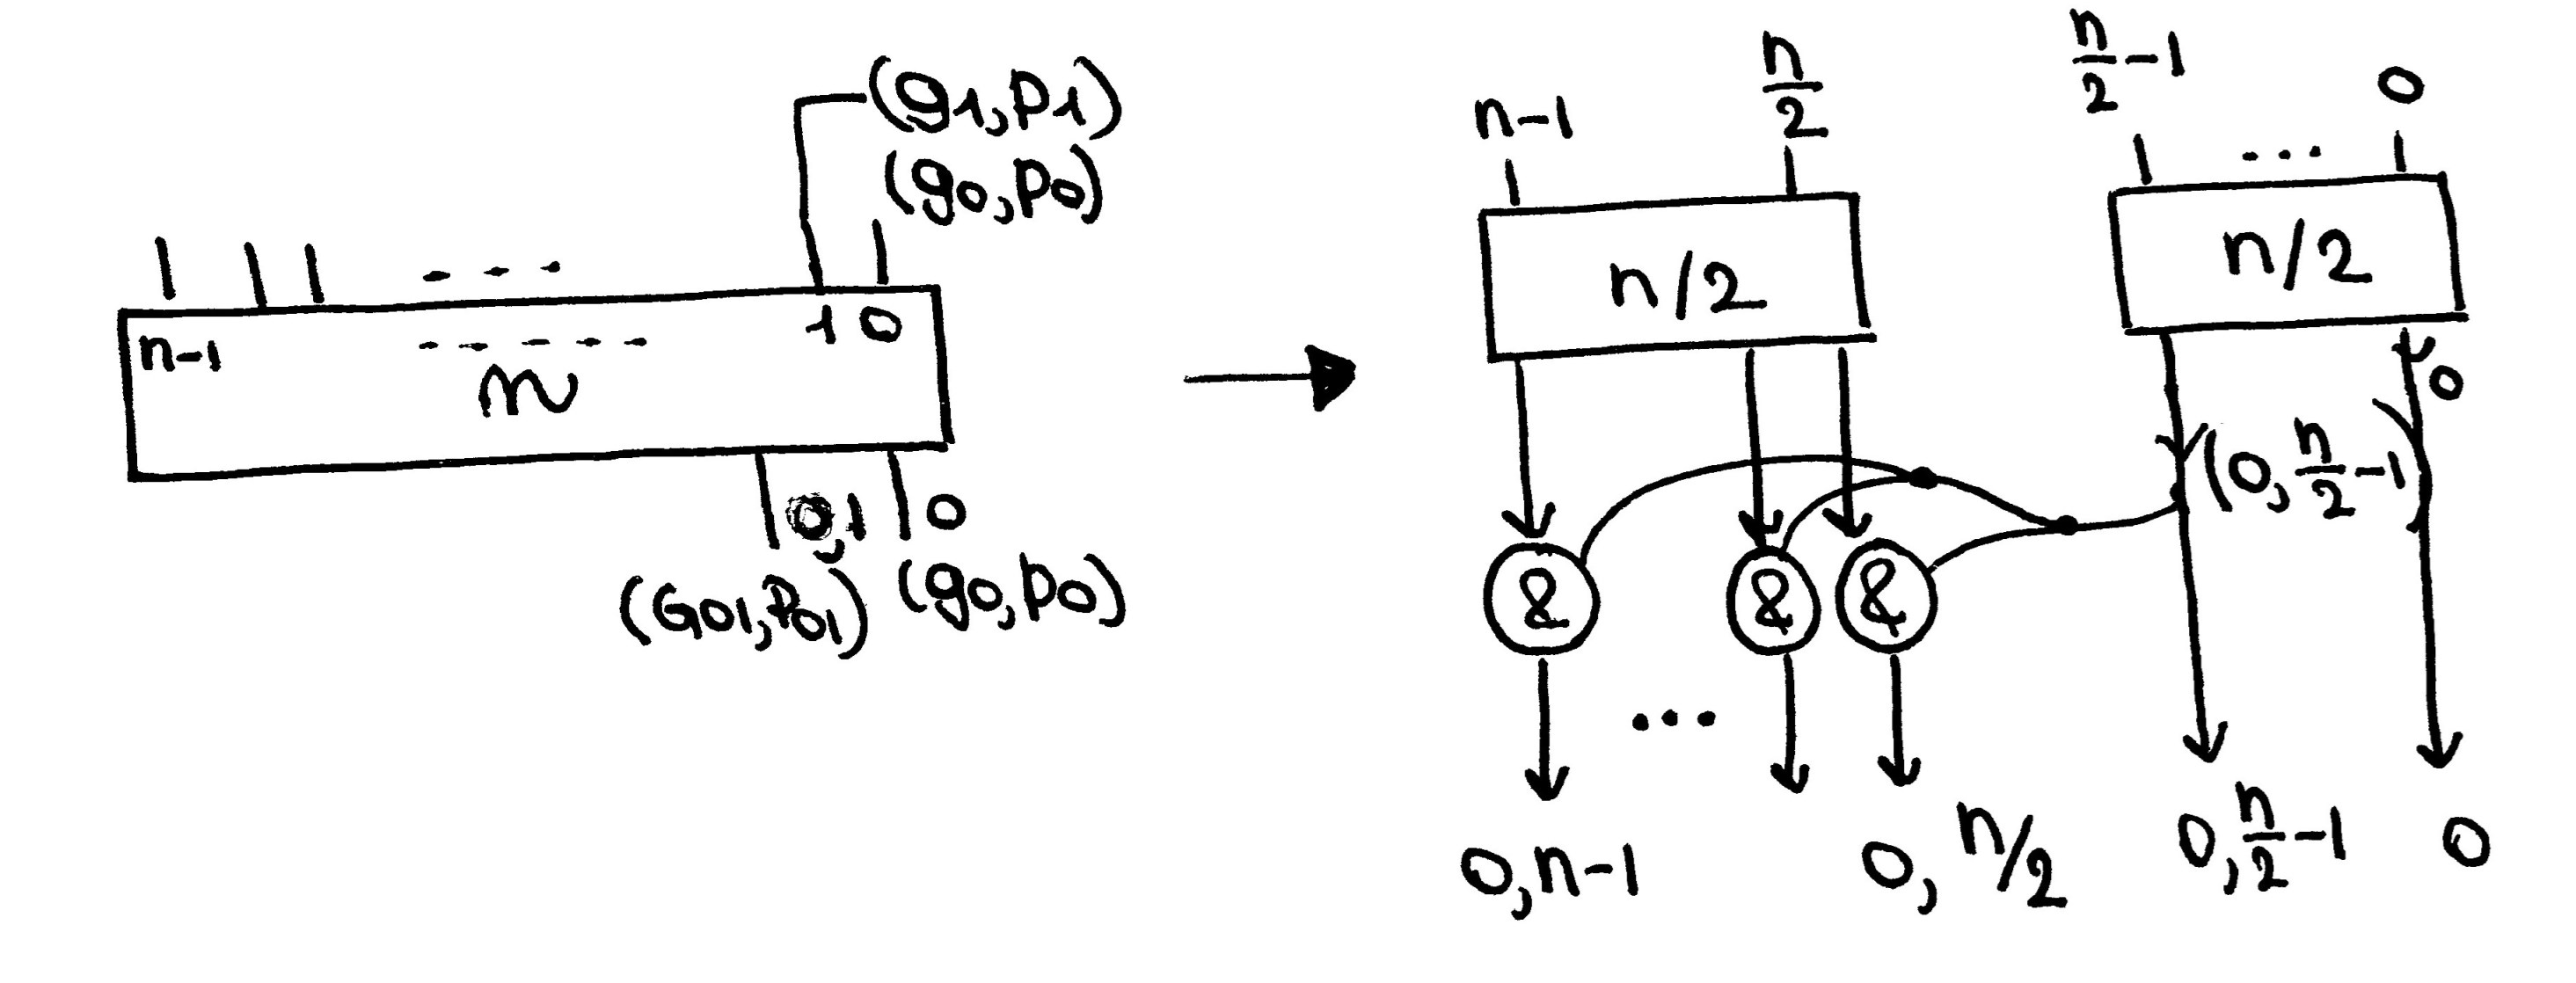
\includegraphics[width=0.7\linewidth]{img/img2/20}
\end{center}
Input set is made up of $n$ samples (for us in position 0 there will be $(g_0, p_0)$) and we expect $n$ outputs where in position 0 there will be just $(g_0, p_0)$, in position 1 (or better (0,1)) we expect $(G_{0,1}, P_{0,1})$ up to last position $(0, n-1)$ corresponding to $(G_{0,n-1}, P_{0,n-1})$.

With this method we split the problem into smaller ones, in the first step we divide the data into 2 blocks, half on one side and half on the other. The first block already gives us a result which is correct, but the second block is proving us data ranging $(n/2, i)$ so starting index is not 0. By combining the first range to the second one using \& operator and replicating this procedure for all subsequent positions, we need to allocate n/2 \& and merge the output of second block with last output of first block.
This is a first solution, then we can allocate for the first block another two blocks each one of n/4 elements and obviously other \& operators.\\

Applying this techniques to $n=8$:

\begin{center}
  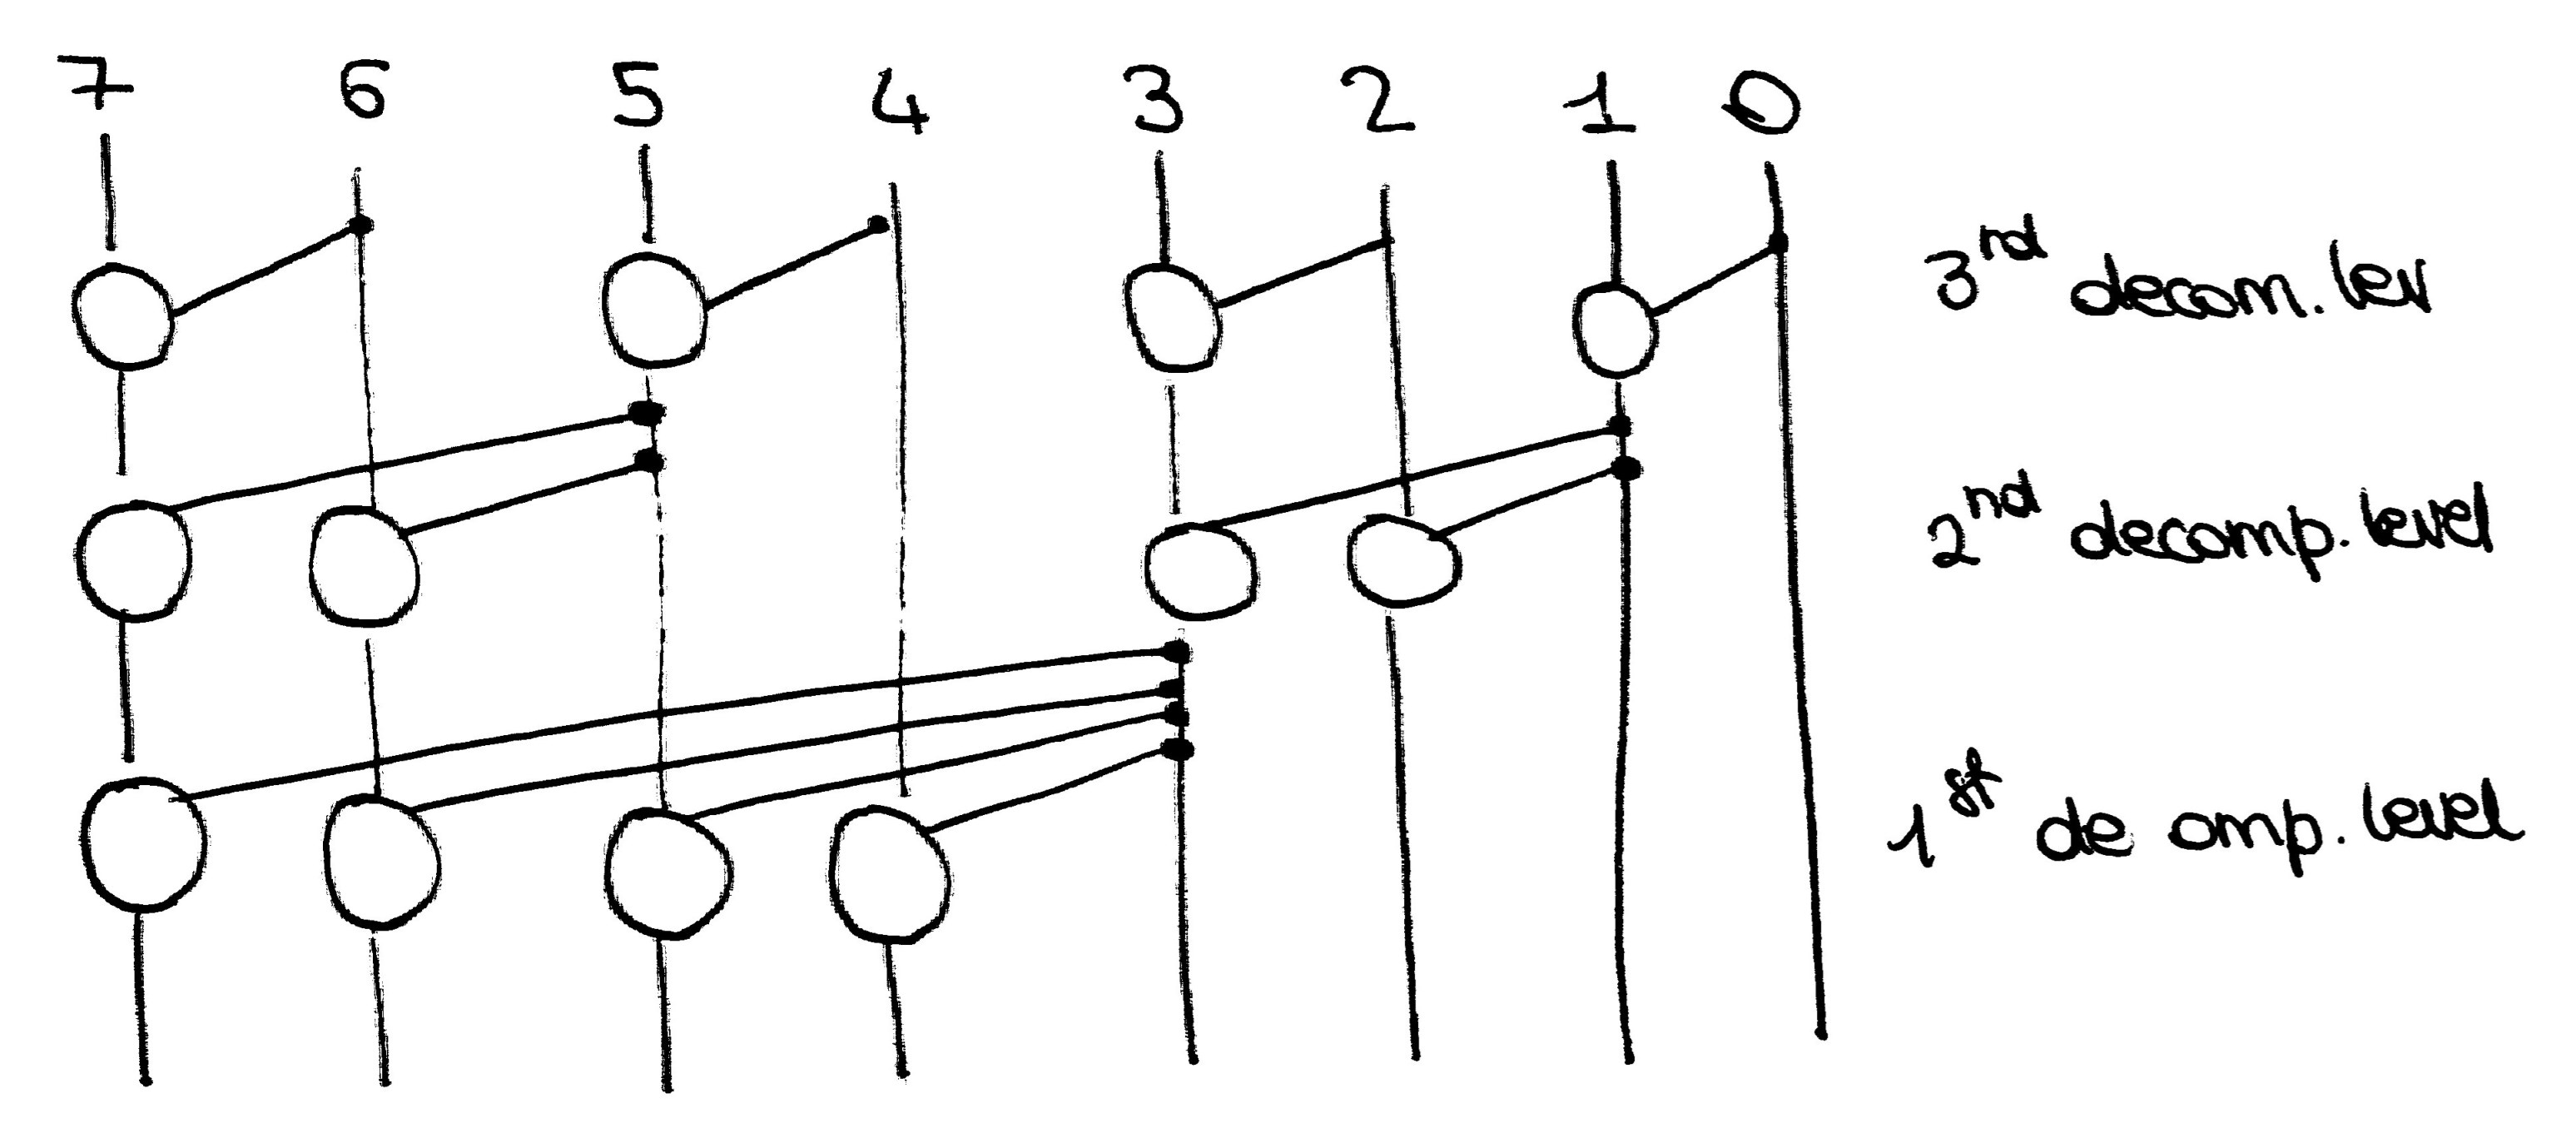
\includegraphics[width=0.7\linewidth]{img/img2/21}
\end{center}

In first level we put all \& between two consecutive inputs making up the third level of decomposition, in second level we start to merge two by two (second level of decomposition)
and in third level the first part is fine while the second part has to be merged with the last outputs of second block, realizing in this way the first level of decomposition.

\subparagraph{Performances evaluation}
\textit{Warning: this is not the complete adder, it only generates G,P starting from g,p but it is actually the most complex part}.\\

\begin{itemize}
  \item \textbf{Complexity} : $ C(n) = $ \#level $\cdot$ \# processing Elements For Each Block $=log_2 (n) \cdot \frac{n}{2}$, so complexity increases linearly with n.
  \item \textbf{Delay} : $ t(n) = $ \# process element we have to go through the critical path = \# levels $= t_{pe} \cdot log_2(n)  $, fine it increases logarithmically.
  \item \textbf{Fan out} : $ F(n) = $ \# process elements that have to be driven from a single point = $= \frac{n}{2}   $, fine it increases logarithmically.

\end{itemize}

Although delay seems to be very low, if $n$ increases in real implementation speed tends to be rather low due to fanout. It seems to be a good solution but with some problems regarding fanout.

%%%%%%%%%%%%%%%%%%%%%%%%%%%%%%%%%%%%%%%%%%%%%%%%%%%%%%%%%%%%%%%%%%%%%%%%%%%%%%%%
%%%%%%%%%%%%%%%%%%%%%%%%%%%%%%%%%%%%%%%%%%%%%%%%%%%%%%%%%%%%%%%%%%%%%%%%%%%%%%%%
%%%%%%%%%%%%%%%%%%%%%%%%%%%%%%%%%%%%%%%%%%%%%%%%%%%%%%%%%%%%%%%%%%%%%%%%%%%%%%%%

\subsection{Brent - Kung}
As before a decomposition of the big problem is performed:

\begin{center}
  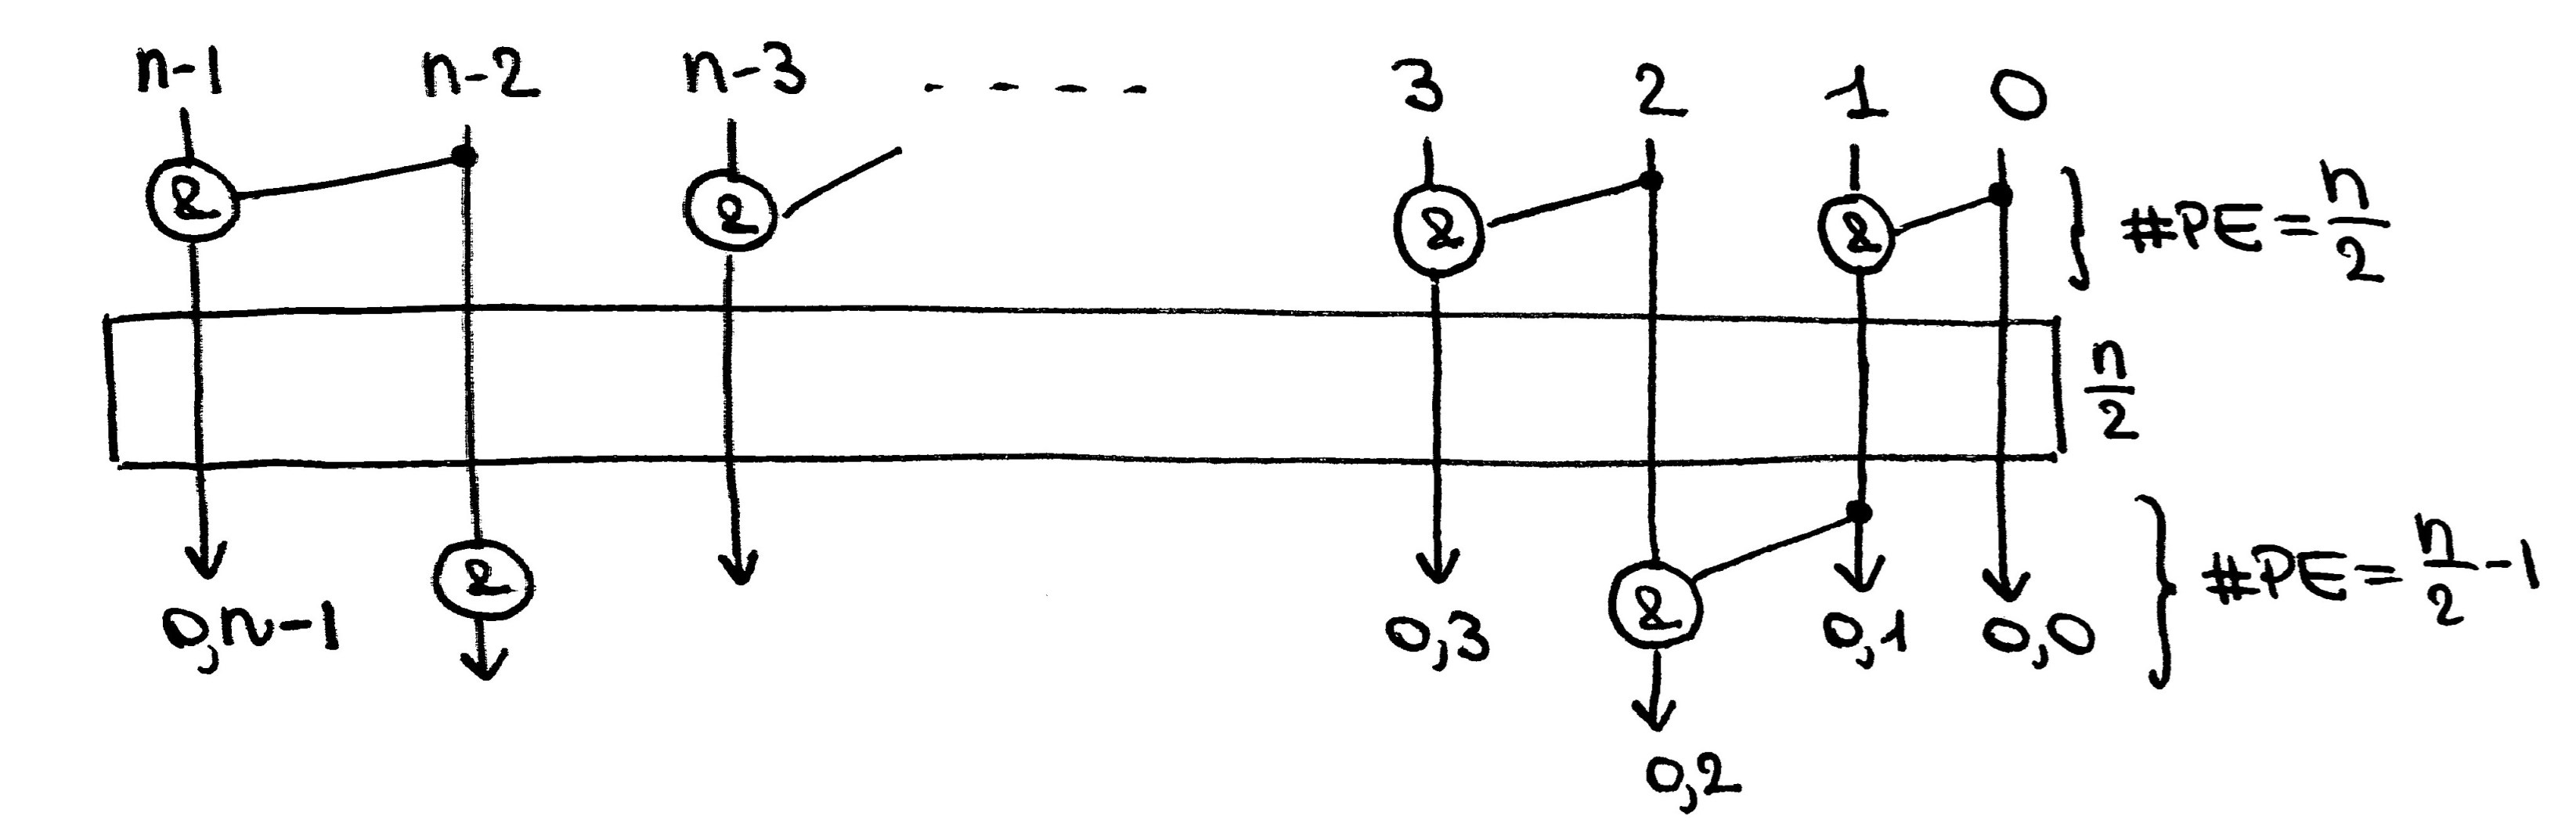
\includegraphics[width=0.7\linewidth]{img/img2/22}
\end{center}

Let's propagate all element in even position while the ones in odd position are processed by a block receiving n/2 inputs (instead of take the first n/2 data, we take one data yes and one not). At the output of inner block we expect (0,1) but we actually have only the first input, so before the input we have to allocate a processing element to merge 0 and 1. For the data in position 2 we need to insert a processing element after the inner block to merge with the output of previous block. This architecture can be completed adding process elements before or after the inner block (before for odd position, after for even position except position 0).\\

The number of processing element we have to allocate for each level of decomposition is $(\frac{n}{2}) + ( \frac{n}{2} -1)$ (before and after inner block). Referring to a complete example:

\begin{center}
  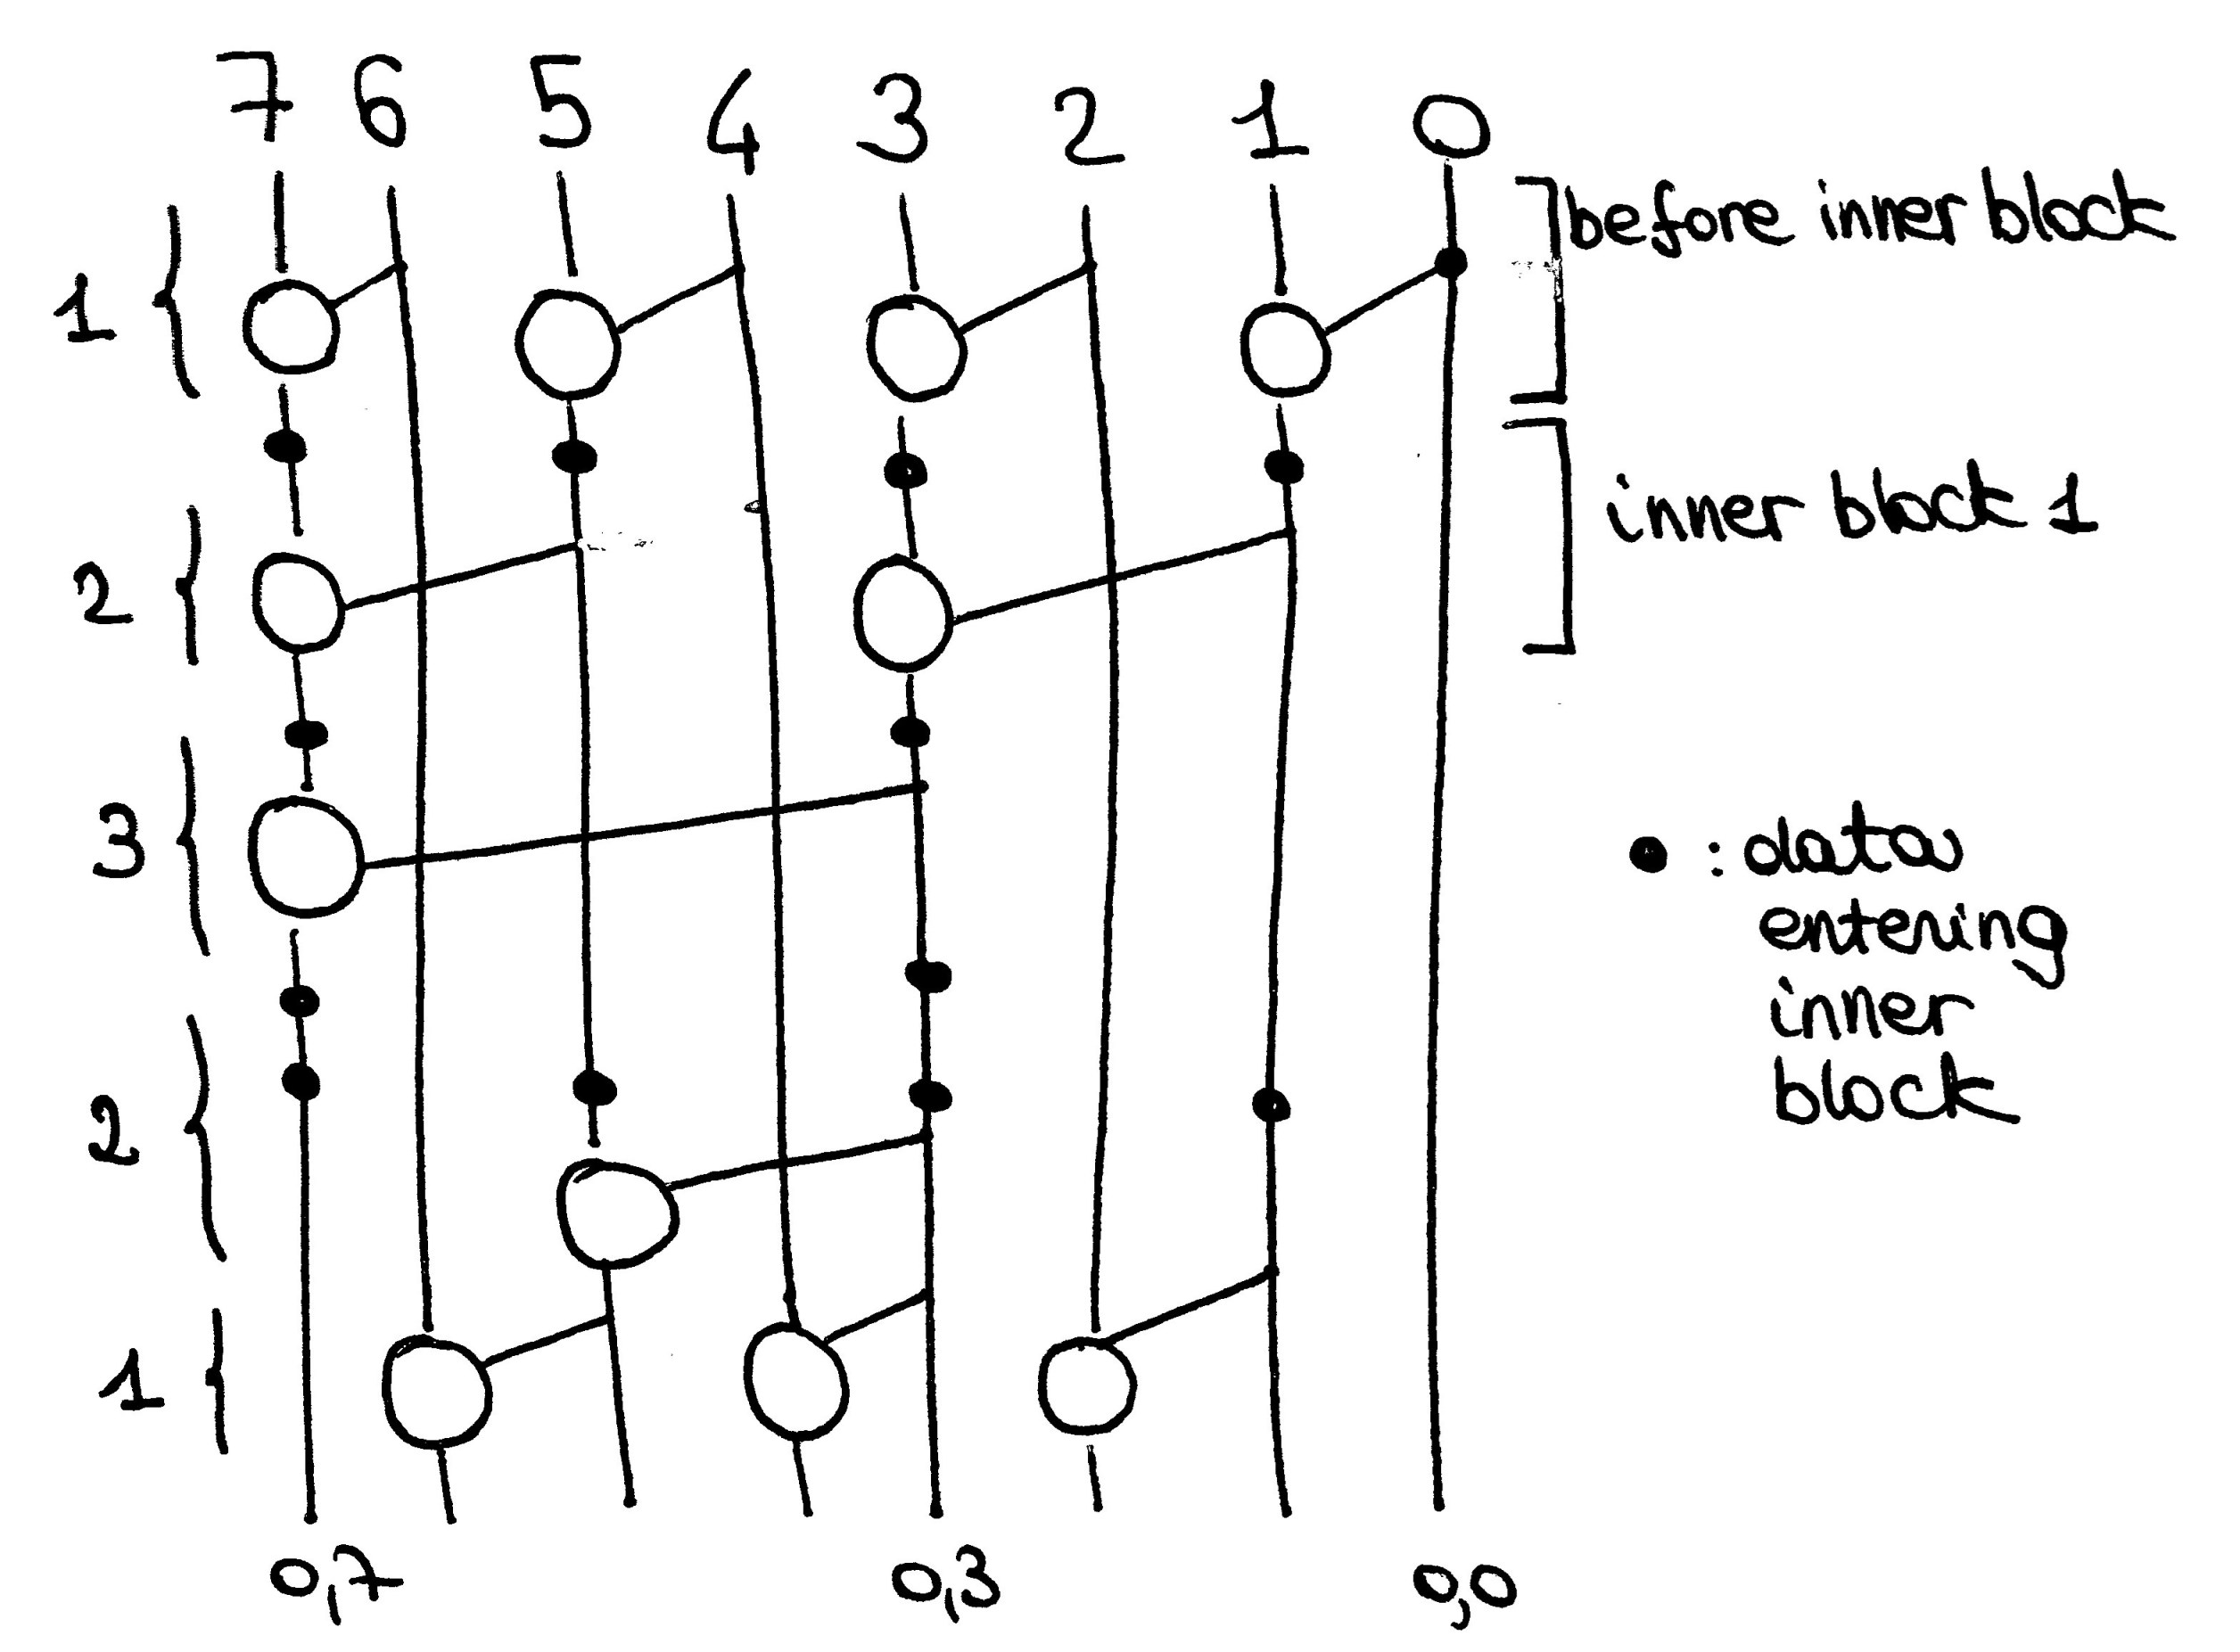
\includegraphics[width=0.7\linewidth]{img/img2/23}
\end{center}

For the second decomposition level no block has to be added at the output, for the first decomposition level we have to place process elements at outputs in even position expect for position zero. Looking at output in position 0 it is already fine, in position 1 we have to combine 0 and 1, in position 2 is fine and so on.

\subparagraph{Performances evaluation}
Regarding complexity, it is:
\begin{eqnarray}
C(n)=C(n/2)+ \#PEs included= C(n/2)+ (n-1)\\
C(n/2)=C(n/4)+(n/2 - 1)\\
..\\
c(n/2^i)=C(n/2^{i-1})+ \frac{n}{2^i}-1\\
\end{eqnarray}

If $k$ is the number of decomposition level, i.e. $k=log_2 n$ then:

$$C(n)=\sum_{i=1}^{k}(\frac{n}{2^i}-1)= n \sum_{i=1}^{k} 2^{-i}-k= 2n-log_2( n) - 2$$

So for $n=8$ $C(n)=11$ (which is one obtained), with respect to Fischer method it's better since it's working as $2n$ and not $nlog_2 n$. For time delay:

$$t(n)=(t_(\frac{n}{2}) + 1 + 1) \cdot (\#innerBlocks -1) = 2log_2 (n) -2$$

Last inner block is not inside the critical path since cp is in the middle. With respect to the previous one, it goes as $2 log$ so it seems worst but looking at fan out:

$$F(n)=log_2 (n)$$

here the fanout is no more increasing linearly.

%%%%%%%%%%%%%%%%%%%%%%%%%%%%%%%%%%%%%%%%%%%%%%%%%%%%%%%%%%%%%%%%%%%%%%%%%%%%%%%%
%%%%%%%%%%%%%%%%%%%%%%%%%%%%%%%%%%%%%%%%%%%%%%%%%%%%%%%%%%%%%%%%%%%%%%%%%%%%%%%%
%%%%%%%%%%%%%%%%%%%%%%%%%%%%%%%%%%%%%%%%%%%%%%%%%%%%%%%%%%%%%%%%%%%%%%%%%%%%%%%%

\subsection{Summarizing}
There are also other networks to solve this problem, summing up together:

\begin{center}
  \begin{tabular}{|l|c|c|c|}
    \hline
    Network&      C(n)&     t(n)&     F(n)\\
    \hline
    Lodner-Fischer&   $0.5nlog_2n$&   $log_2n$&   $n/2$\\
    Brent-Kogge &   $2n-2-log_2n$&    $2log$&     $log_2 n$\\
    Kogge Stone &   $nlog_2n - n+1$&   $log_2$&     $log_2 n$\\
    \hline
  \end{tabular}
\end{center}


In terms of delay only 1 and 3 are the best one, but considering also fanout just last one is better. Looking at complexity the best one is the first one. Depending on technology, we can choose the best one.

%%%%%%%%%%%%%%%%%%%%%%%%%%%%%%%%%%%%%%%%%%%%%%%%%%%%%%%%%%%%%%%%%%%%%%%%%%%%%%%%
%%%%%%%%%%%%%%%%%%%%%%%%%%%%%%%%%%%%%%%%%%%%%%%%%%%%%%%%%%%%%%%%%%%%%%%%%%%%%%%%
%%%%%%%%%%%%%%%%%%%%%%%%%%%%%%%%%%%%%%%%%%%%%%%%%%%%%%%%%%%%%%%%%%%%%%%%%%%%%%%%

\section{Multi-operand adders}

In this situation we are required to sum together partial products or consecutive samples like in a filter, therefore in multipliers and filter multi-operand adders are used. In general we want to sum together $k$ operands each one represented on $n$ bits.

\subparagraph{I idea: sequentially process}
\begin{center}
  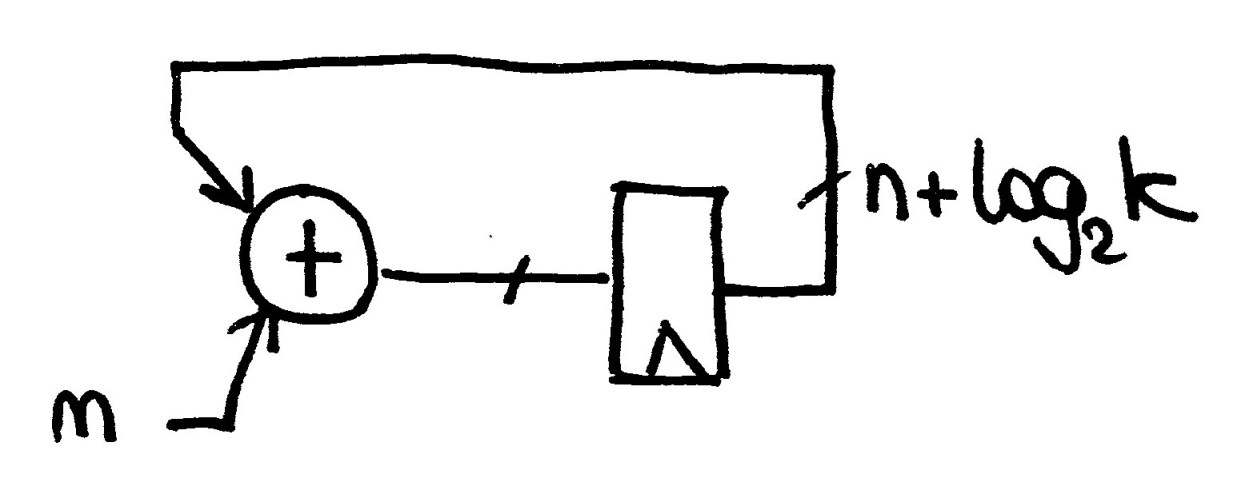
\includegraphics[width=0.5\linewidth]{img/img2/24}
\end{center}

Register and adder have to be sized for the worst case, which is $n+log_2(k)$. An estimation of the total time required is $k(n+log_2(k))$ assuming for adder a RCA.

\subparagraph{II idea: tree-like form  (or in parallel)}
\begin{center}
  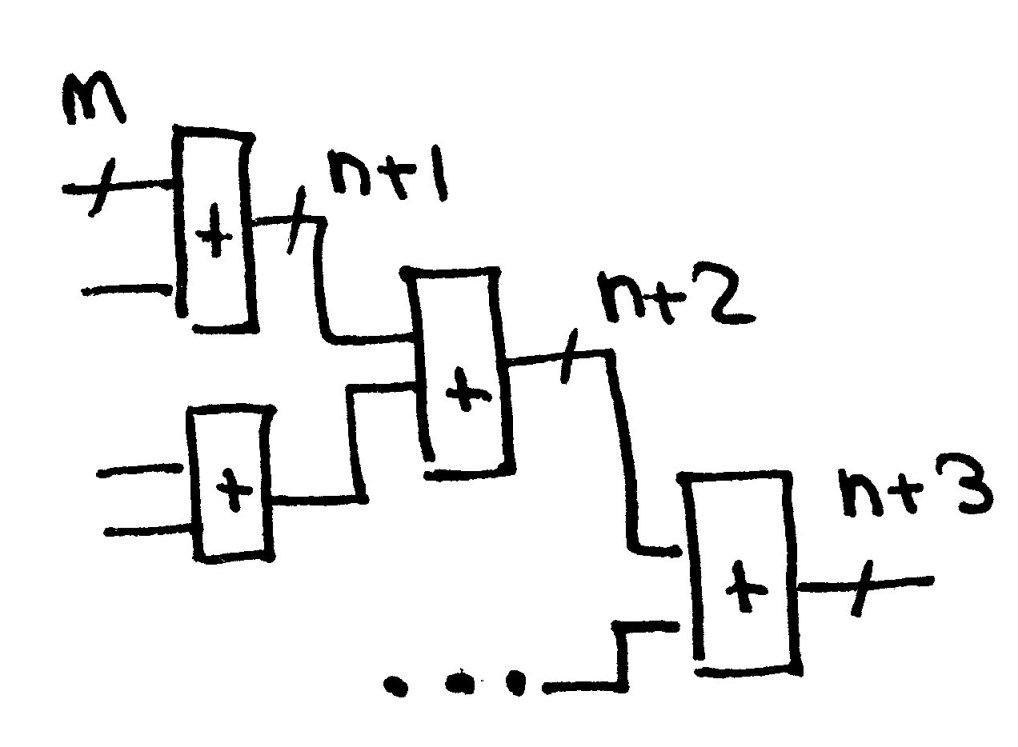
\includegraphics[width=0.5\linewidth]{img/img2/25}
\end{center}

To evaluate critical path we don't have to compute delay adder 1 + delay adder 2+... etc because the adder at second level can start its work when the two least sign bit of the first level are available, meaning that:
$t_{start,1}=0$\\
$t_{start,2}=1$ (1 full adder delay)\\
$t_{start,3}=2$\\
$...$\\

So with $log_2( k)$ levels the last one has to wait for all the previous adder, so along the critical path there are $2log_2 (k)+n$ full adders. This approach is better than sequential one.

%%%%%%%%%%%%%%%%%%%%%%%%%%%%%%%%%%%%%%%%%%%%%%%%%%%%%%%%%%%%%%%%%%%%%%%%%%%%%%%%
%%%%%%%%%%%%%%%%%%%%%%%%%%%%%%%%%%%%%%%%%%%%%%%%%%%%%%%%%%%%%%%%%%%%%%%%%%%%%%%%
%%%%%%%%%%%%%%%%%%%%%%%%%%%%%%%%%%%%%%%%%%%%%%%%%%%%%%%%%%%%%%%%%%%%%%%%%%%%%%%%

\section{Carry save adder (CSA)}

The key idea is to use a full adder as compressor. Let's take a full adder, all inputs are at the same level meaning that they all have the same weight ($a_i,b_i, c_i$) instead for outputs $s_i$ has a weight equal to $2^i$ while carry out has a weight equal to $2^{i+1}$ so it has to be aligned to next full adder.

\begin{center}
  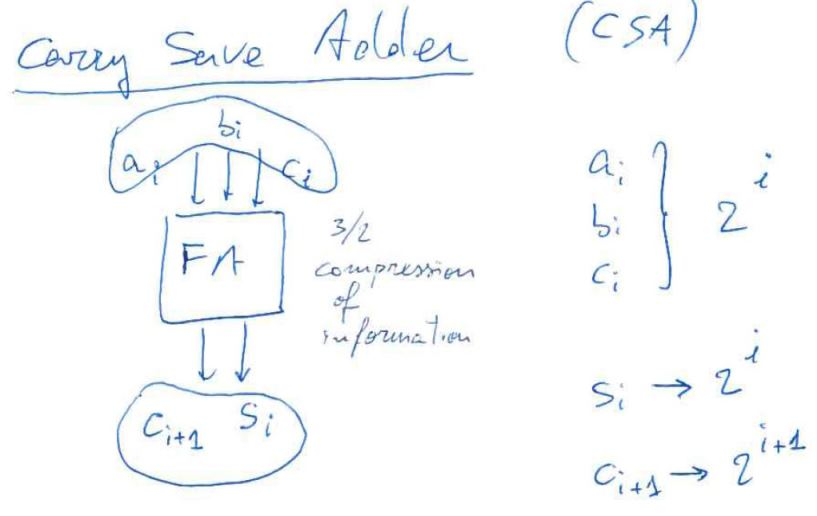
\includegraphics[width=0.7\linewidth]{img/img2/26}
\end{center}
\begin{center}
  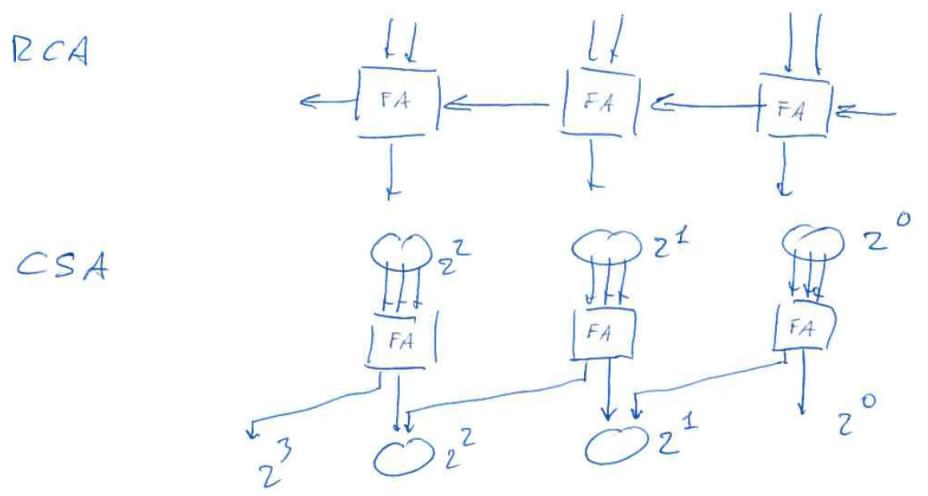
\includegraphics[width=0.7\linewidth]{img/img2/27}
\end{center}

\subparagraph{Example}
\begin{verbatim}
img30














\end{verbatim}
In this case it is $k=7$ so there are 7 operands to be added together (these operands are not on 1 bit only) so we start by adding the first 3 using a CSA (compression of information). Then we take 3 more inputs and the remaining one has to be forwarding with no changes. At the output of CSA we will have 2 stream/CSA. By inserting 4 CSA levels at the end we can obtain only two outputs that can be delivered to a classing 2-input adder.\\

In general if $h$ is the amount of levels needed to deal with $k$ elements, $h(k)$ can be expresses as:
$$h(7)=1+h(\lceil \frac{2}{3}7 \rceil )=1+h(5)$$
where:
\begin{eqnarray}
h(5)=1+h(\lceil \frac{2}{3}5 \rceil )=1+h(4)\\
h(4)=1+h(\lceil \frac{2}{3}4 \rceil )=1+h(3)\\
h(3)=1+h(\lceil \frac{2}{3}3 \rceil )=1+h(2)\\
\end{eqnarray}

since $h(2)=0$ because we don't need anymore a CSA. Every level is introducing a delay equal to the one of a single full adder but we don't have to forget last adder.
Each CSA is a compressor from 3 to 2 so the number of operands decreases as 2/3, integer part.\\

Introducing dot notation we associate the weight of a bit in a certain operand. So in a 7 operand adder, we can describe the operation to be performed as:
$k=7$ is the number of operands while $n=6$ is the parallelism of each operand.
We have to combine bits with same weight, so same weight means same column. Each full adder gives us 1 sum bit which has the same weight as the input plus carry out. For the first level of compression we have sum bit + carry out of the first 2 groups of 3 bit + the last row.
For second level of compression we do the same thing, so if the number of rows is greater than 2 we can continue to compress it.
At third level we see that for the last column we would introduce an additional level of CSA since the carry out of the last CSA would be combined with the other two bits. To avoid it we can use a half adder (the one in dot) to combine two bits which will stay with last carry out. This half adder is not acting as a compressor (2 input, 2 output) but it avoids to have 3 points in the penultimate column. At the end we need:

\begin{center}
  \begin{tabular}{|l|c|c|}
    \hline
    Level&  FAs&  HAs\\
    \hline
    I&    12&   0\\
    II&   6&    0\\
    III&  6&    0\\
    IV&   4&    1\\
    V(RCA)& 5&    2\\
    \hline
  \end{tabular}
\end{center}

Total delay is equal to delay of final RCA plus CSA tree delay (which is equal to number of level multiply the delay of a FA). There are multiple possibilities to distribute FA and HA in the tree, we will do it better when talking on multipliers (Wallace approach: asap allocation of CSA, Dadda approach: a little bit different).

\begin{center}
  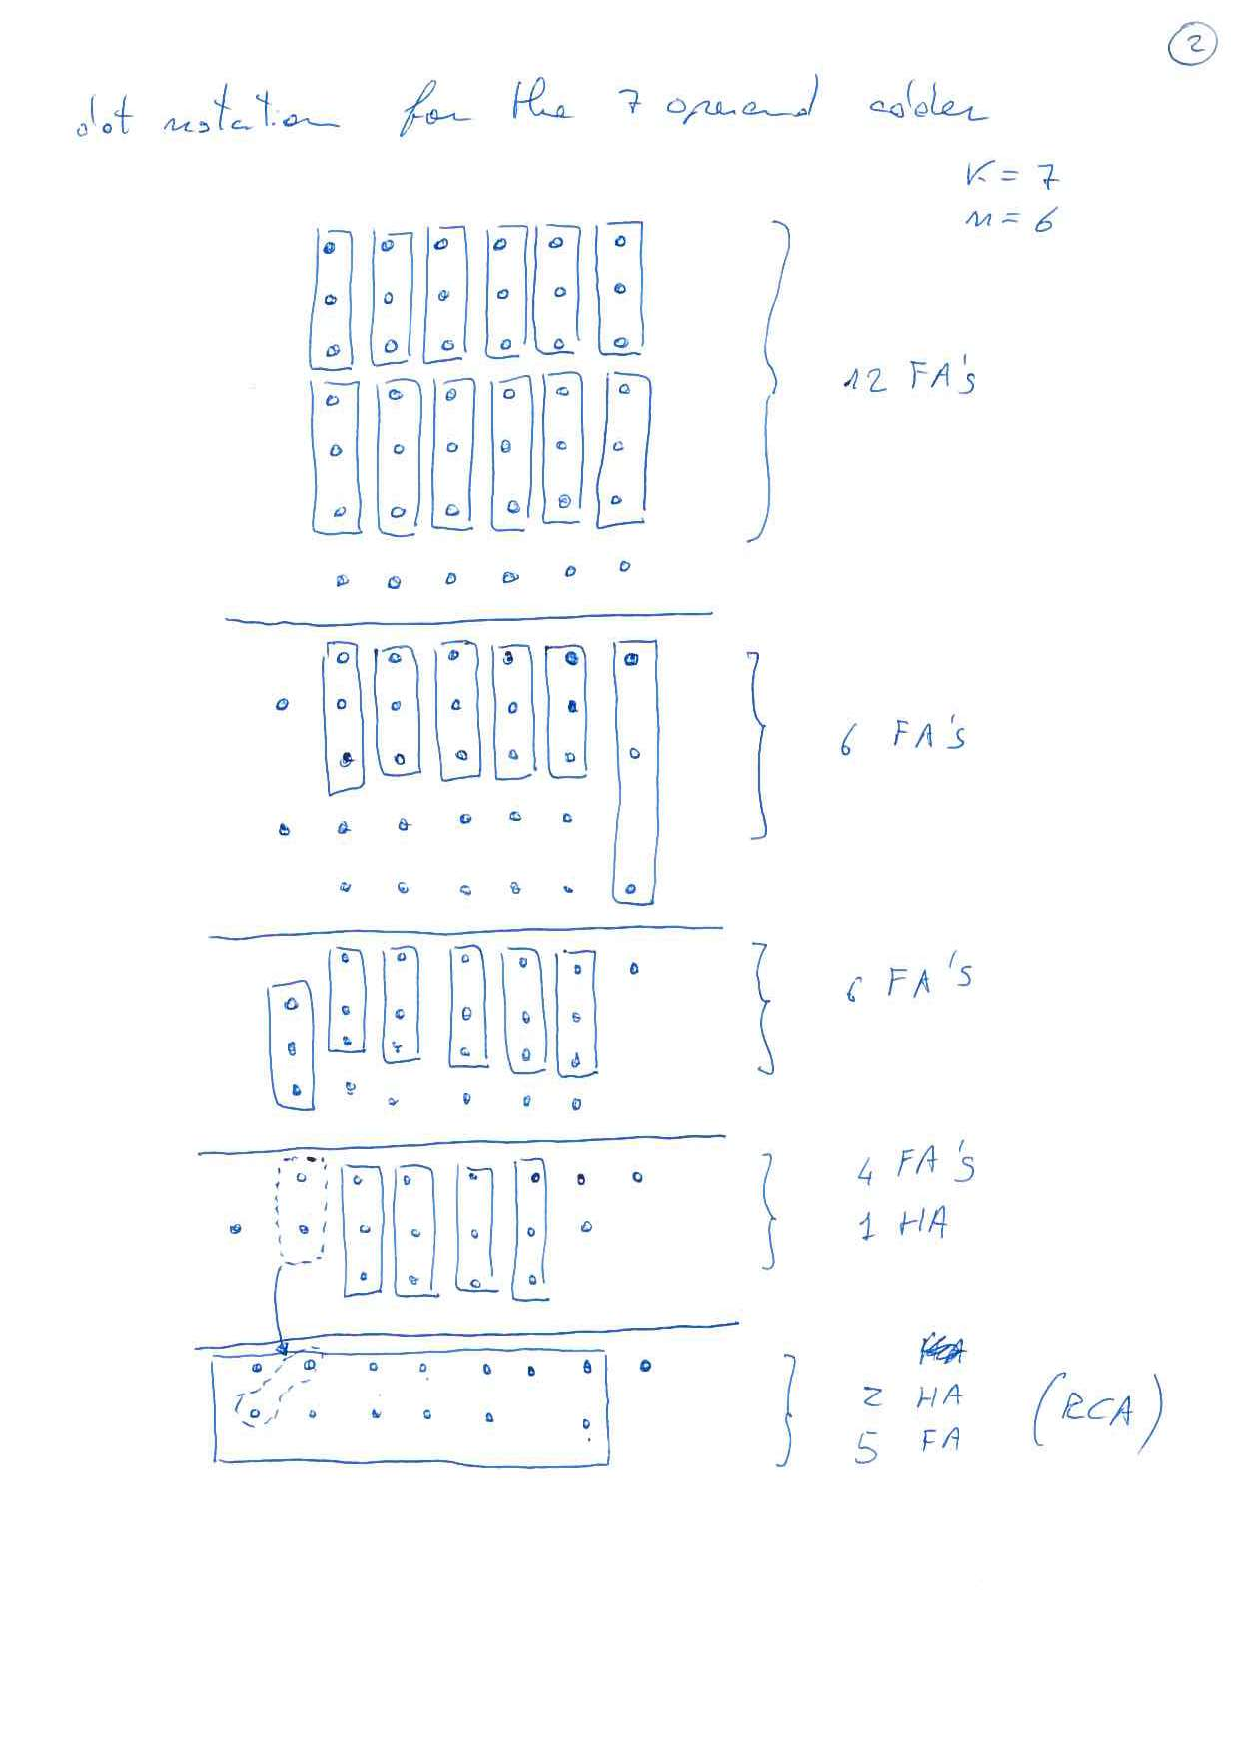
\includegraphics[width=1.0\linewidth]{img/img2/31}
\end{center}

